\documentclass[11pt,oneside,openany]{book}

% A visual, self-contained mathematics roadmap.
\usepackage[a4paper,margin=1.62cm,headheight=14pt,footskip=0.72cm]{geometry}
\usepackage[T1]{fontenc}
\usepackage[utf8]{inputenc}
\usepackage{lmodern}
\usepackage{microtype}
\usepackage{amsmath,amssymb,mathtools}
\usepackage{booktabs,array,multirow}
\usepackage{enumitem}
\usepackage{xcolor}
\usepackage{tikz}
\usetikzlibrary{arrows.meta,calc,decorations.pathreplacing,patterns,positioning,angles,quotes,3d,fit,matrix,shapes.geometric}
\usepackage{pgfplots}
\pgfplotsset{compat=1.18}
\usepgfplotslibrary{fillbetween}
\usepackage[most]{tcolorbox}
\usepackage{multicol}
\usepackage{titlesec}
\usepackage{fancyhdr}
\usepackage{hyperref}
\usepackage{bookmark}

% Palette
\definecolor{ink}{HTML}{18212B}
\definecolor{muted}{HTML}{5F6B76}
\definecolor{blue}{HTML}{1769AA}
\definecolor{bluepale}{HTML}{EAF4FB}
\definecolor{teal}{HTML}{087F8C}
\definecolor{tealpale}{HTML}{E8F7F7}
\definecolor{orange}{HTML}{C56A12}
\definecolor{orangepale}{HTML}{FFF4E5}
\definecolor{purple}{HTML}{6C4AB6}
\definecolor{purplepale}{HTML}{F2EEFF}
\definecolor{green}{HTML}{2C7A4B}
\definecolor{greenpale}{HTML}{EBF7EF}
\definecolor{linegray}{HTML}{D9E0E6}

\color{ink}
\hypersetup{colorlinks=true,linkcolor=blue,urlcolor=teal,citecolor=purple,hypertexnames=false,pdftitle={Mathematics From Zero: A Visual Roadmap},pdfauthor={Scott Brodie Forsyth}}
\setlength{\parindent}{0pt}
\setlength{\parskip}{0.52em}
\setlist[itemize]{leftmargin=1.35em,itemsep=0.18em,topsep=0.2em}
\setlist[enumerate]{leftmargin=1.5em,itemsep=0.18em,topsep=0.2em}

\titleformat{\chapter}[display]
  {\normalfont\bfseries\color{blue}}
  {\fontsize{13}{16}\selectfont\chaptertitlename\ \thechapter}
  {0.35em}{\fontsize{30}{34}\selectfont}
  [\vspace{0.35em}\color{teal}\titlerule]
\titlespacing*{\chapter}{0pt}{-10pt}{20pt}
\titleformat{\section}{\normalfont\Large\bfseries\color{blue}}{\thesection}{0.55em}{}
\titleformat{\subsection}{\normalfont\large\bfseries\color{teal}}{\thesubsection}{0.5em}{}

\pagestyle{fancy}
\fancyhf{}
\fancyhead[L]{\small\textcolor{muted}{Mathematics From Zero}}
\fancyhead[R]{\small\textcolor{muted}{\leftmark}}
\fancyfoot[C]{\small\textcolor{muted}{\thepage}}
\renewcommand{\headrulewidth}{0.35pt}
\renewcommand{\chaptermark}[1]{\markboth{#1}{}}

\newtcolorbox{conceptbox}[1]{enhanced,breakable,colback=bluepale,colframe=blue!65!black,colbacktitle=blue!65!black,coltitle=white,boxrule=0.65pt,arc=2mm,left=2.2mm,right=2.2mm,top=1.5mm,bottom=1.5mm,fonttitle=\bfseries,title={#1}}
\newtcolorbox{intuitionbox}[1]{enhanced,breakable,colback=tealpale,colframe=teal!65!black,colbacktitle=teal!65!black,coltitle=white,boxrule=0.65pt,arc=2mm,left=2.2mm,right=2.2mm,top=1.5mm,bottom=1.5mm,fonttitle=\bfseries,title={#1}}
\newtcolorbox{warningbox}[1]{enhanced,breakable,colback=orangepale,colframe=orange!75!black,colbacktitle=orange!75!black,coltitle=white,boxrule=0.65pt,arc=2mm,left=2.2mm,right=2.2mm,top=1.5mm,bottom=1.5mm,fonttitle=\bfseries,title={#1}}
\newtcolorbox{proofbox}[1]{enhanced,breakable,colback=purplepale,colframe=purple!65!black,colbacktitle=purple!65!black,coltitle=white,boxrule=0.65pt,arc=2mm,left=2.2mm,right=2.2mm,top=1.5mm,bottom=1.5mm,fonttitle=\bfseries,title={#1}}
\newtcolorbox{checkpointbox}[1]{enhanced,breakable,colback=greenpale,colframe=green!65!black,colbacktitle=green!65!black,coltitle=white,boxrule=0.65pt,arc=2mm,left=2.2mm,right=2.2mm,top=1.5mm,bottom=1.5mm,fonttitle=\bfseries,title={#1}}

\newcommand{\R}{\mathbb{R}}
\newcommand{\N}{\mathbb{N}}
\newcommand{\Z}{\mathbb{Z}}
\newcommand{\Q}{\mathbb{Q}}
\newcommand{\C}{\mathbb{C}}
\newcommand{\vect}[1]{\boldsymbol{#1}}
\newcommand{\dd}{\,\mathrm{d}}
\newcommand{\abs}[1]{\left|#1\right|}
\newcommand{\norm}[1]{\left\lVert#1\right\rVert}
\newcommand{\set}[1]{\left\{#1\right\}}
\newcommand{\floor}[1]{\left\lfloor#1\right\rfloor}
\newcommand{\ceil}[1]{\left\lceil#1\right\rceil}
\newcommand{\unit}[1]{\,\mathrm{#1}}
\newcommand{\todo}[1]{\textcolor{orange}{[\textit{#1}]}}

\newenvironment{definition}{\begin{conceptbox}{Definition}}{\end{conceptbox}}
\newenvironment{example}{\begin{intuitionbox}{Worked example}}{\end{intuitionbox}}
\newenvironment{keyidea}{\begin{checkpointbox}{Key idea}}{\end{checkpointbox}}

\begin{document}

\begin{titlepage}
\thispagestyle{empty}
\begin{tikzpicture}[remember picture,overlay]
  \fill[blue] (current page.north west) rectangle ([yshift=-5.45cm]current page.north east);
  \fill[teal] ([yshift=-5.45cm]current page.north west) rectangle ([yshift=-5.60cm]current page.north east);
  \foreach \x in {0,...,15}{
    \draw[white,opacity=0.13,line width=0.45pt] ([xshift=\x cm,yshift=-0.4cm]current page.north west) -- ([xshift=\x cm,yshift=-5.15cm]current page.north west);
  }
  \foreach \y in {0,...,4}{
    \draw[white,opacity=0.13,line width=0.45pt] ([xshift=0.2cm,yshift=-\y cm-0.7cm]current page.north west) -- ([xshift=20cm,yshift=-\y cm-0.7cm]current page.north west);
  }
  \node[anchor=west,text=white,font=\fontsize{28}{32}\selectfont\bfseries,align=left]
    at ([xshift=1.6cm,yshift=-1.15cm]current page.north west) {Mathematics\\[-1pt]From Zero};
  \node[anchor=west,text=white!86,font=\large]
    at ([xshift=1.65cm,yshift=-4.35cm]current page.north west) {A visual roadmap from counting to structure};
  \node[anchor=north east,text=white,font=\large\bfseries]
    at ([xshift=-1.6cm,yshift=-1.2cm]current page.north east) {A visual roadmap};
\end{tikzpicture}

\vspace*{6.35cm}
{\Large\color{teal}\bfseries See the structure. Then use the symbols.}\par
\vspace{0.65cm}
\rule{0.52\linewidth}{1.2pt}\par
\vspace{0.65cm}
{\large\color{muted} A visual introduction to the language, ideas, and connected\newline tools of mathematics}\par

\vfill
\begin{center}
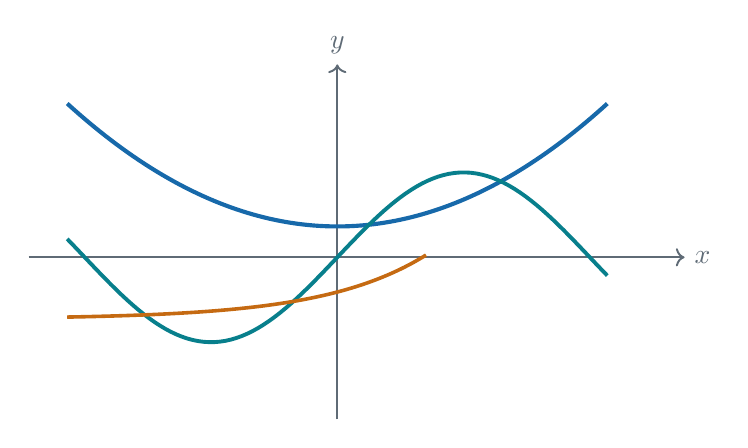
\begin{tikzpicture}[scale=0.98]
  \draw[->,line width=0.7pt,muted] (-4,0) -- (4.5,0) node[right] {$x$};
  \draw[->,line width=0.7pt,muted] (0,-2.1) -- (0,2.5) node[above] {$y$};
  \draw[blue,line width=1.5pt,samples=100,domain=-3.5:3.5] plot (\x,{0.13*\x*\x+0.4});
  \draw[teal,line width=1.4pt,samples=100,domain=-3.5:3.5] plot (\x,{1.1*sin(55*\x)});
  \draw[orange,line width=1.3pt,samples=100,domain=-3.5:1.15] plot (\x,{0.35*exp(0.75*\x)-0.8});
\end{tikzpicture}
\end{center}

\vfill
{\large\bfseries Scott Brodie Forsyth}\par
{\color{muted} 2026}
\end{titlepage}

\frontmatter
\chapter*{A note before we begin}
\addcontentsline{toc}{chapter}{A note before we begin}

This is a visual map of core mathematics. It is designed for a reader who may remember almost nothing from school, but who wants to build toward university-level mathematics, statistics, computing, economics, or science.

No single book can contain literally every mathematical concept. Mathematics branches into thousands of specialised subjects. This book therefore focuses on the central trunk and the major branches: the ideas that recur across algebra, geometry, calculus, probability, statistics, linear algebra, discrete mathematics, differential equations, and proof. Each topic starts with a picture or mental model, then introduces notation, then shows how the pieces connect.

\begin{conceptbox}{How to read a page}
\begin{enumerate}
  \item First look at the picture. Ask what changes and what stays fixed.
  \item Read the sentence in plain language before reading the formula.
  \item Translate the formula into a small numerical example.
  \item Try to draw the idea yourself. A rough diagram is often more useful than a memorised rule.
  \item Return later and prove or derive the rule. Understanding grows in layers.
\end{enumerate}
\end{conceptbox}

\begin{keyidea}
Mathematics is not primarily a collection of tricks. It is a way to describe structure: quantity, shape, change, uncertainty, relationships, and the rules that connect them.
\end{keyidea}

\tableofcontents

\chapter*{The map in one page}
\addcontentsline{toc}{chapter}{The map in one page}

\begin{center}
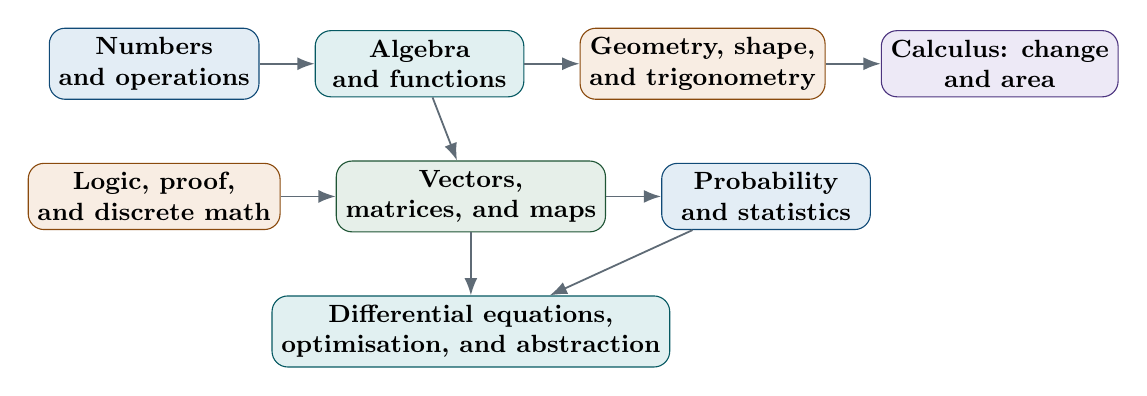
\begin{tikzpicture}[node distance=8mm and 7mm, every node/.style={font=\small\bfseries,align=center},
  box/.style={rounded corners=2mm,draw=#1!70!black,fill=#1!12,minimum width=2.65cm,minimum height=0.82cm},
  arr/.style={-{Latex[length=2.2mm]},draw=muted,line width=0.65pt}]
  \node[box=blue] (num) {Numbers\\and operations};
  \node[box=teal,right=of num] (alg) {Algebra\\and functions};
  \node[box=orange,right=of alg] (geo) {Geometry, shape,\\and trigonometry};
  \node[box=purple,right=of geo] (calc) {Calculus: change\\and area};
  \node[box=orange,below=of num] (proof) {Logic, proof,\\and discrete math};
  \node[box=green,right=of proof] (lin) {Vectors,\\matrices, and maps};
  \node[box=blue,right=of lin] (prob) {Probability\\and statistics};
  \node[box=teal,below=of lin] (adv) {Differential equations,\\optimisation, and abstraction};
  \draw[arr] (num)--(alg);
  \draw[arr] (alg)--(geo);
  \draw[arr] (geo)--(calc);
  \draw[arr] (alg)--(lin);
  \draw[arr] (proof)--(lin);
  \draw[arr] (lin)--(prob);
  \draw[arr] (lin)--(adv);
  \draw[arr] (prob)--(adv);
\end{tikzpicture}
\end{center}

\vspace{0.5em}
The arrows are not a rigid order. They show influence. Algebra describes relationships; geometry gives those relationships a visual home; calculus studies how relationships change; linear algebra turns many-variable relationships into maps; probability and statistics describe uncertainty and evidence; discrete mathematics studies finite structure; and advanced mathematics generalises the same patterns.

\mainmatter

\chapter{The language of quantity}

\section{Numbers are positions, amounts, and labels}

A number can answer different questions. The number $5$ can mean five objects, the location five steps to the right of zero, the result of a measurement, or a label such as a bus route. Mathematics becomes clearer when we keep the role of a number visible.

\begin{center}
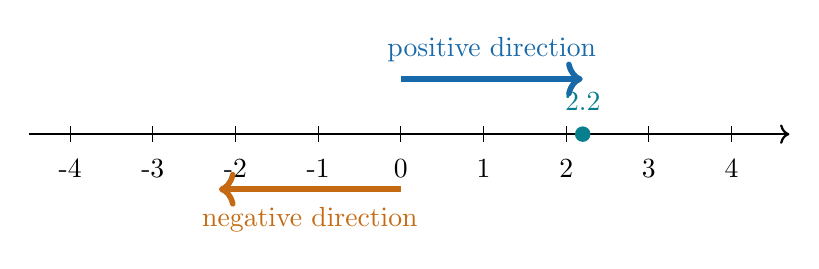
\begin{tikzpicture}[x=1.05cm,y=1cm]
  \draw[->,line width=0.8pt] (-4.5,0)--(4.7,0);
  \foreach \x/\lab in {-4/-4,-3/-3,-2/-2,-1/-1,0/0,1/1,2/2,3/3,4/4}
    {\draw (\x,0.10)--(\x,-0.10) node[below=3pt] {\lab};}
  \draw[blue,line width=2pt,->] (0,0.7)--(2.2,0.7) node[midway,above=2pt] {positive direction};
  \draw[orange,line width=2pt,->] (0,-0.7)--(-2.2,-0.7) node[midway,below=2pt] {negative direction};
  \fill[teal] (2.2,0) circle (2.8pt) node[above=5pt] {$2.2$};
\end{tikzpicture}
\end{center}

\begin{definition}
The natural numbers $\N$ count whole objects. The integers $\Z$ add negatives. The rational numbers $\Q$ are ratios of integers. The real numbers $\R$ fill the entire number line, including numbers such as $\sqrt{2}$ and $\pi$. The complex numbers $\C$ extend the line with a perpendicular imaginary direction.
\end{definition}

\begin{center}
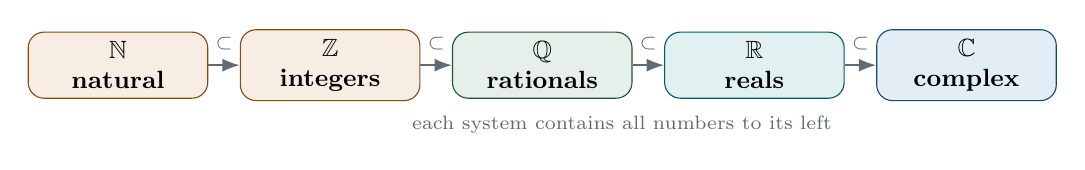
\begin{tikzpicture}[node distance=4mm and 4mm, every node/.style={font=\small\bfseries,align=center},
  sys/.style={rounded corners=2mm,draw=#1!70!black,fill=#1!12,minimum width=2.28cm,minimum height=0.78cm},
  arr/.style={-{Latex[length=2.2mm]},draw=muted,line width=0.65pt}]
  \node[sys=orange] (nat) {$\N$\\natural};
  \node[sys=orange,right=of nat] (int) {$\Z$\\integers};
  \node[sys=green,right=of int] (rat) {$\Q$\\rationals};
  \node[sys=teal,right=of rat] (real) {$\R$\\reals};
  \node[sys=blue,right=of real] (cplx) {$\C$\\complex};
  \draw[arr] (nat)--node[above=2pt,font=\scriptsize,muted] {$\subset$} (int);
  \draw[arr] (int)--node[above=2pt,font=\scriptsize,muted] {$\subset$} (rat);
  \draw[arr] (rat)--node[above=2pt,font=\scriptsize,muted] {$\subset$} (real);
  \draw[arr] (real)--node[above=2pt,font=\scriptsize,muted] {$\subset$} (cplx);
  \node[font=\scriptsize,muted] at (6.4,-0.75) {each system contains all numbers to its left};
\end{tikzpicture}
\end{center}

\section{Operations are transformations}

Addition combines quantities, subtraction compares or reverses addition, multiplication scales or repeats, and division undoes multiplication. The familiar order of operations is a compact way to preserve the structure of a calculation:
\[
  \text{grouping} \quad\longrightarrow\quad \text{powers} \quad\longrightarrow\quad \text{multiplication/division} \quad\longrightarrow\quad \text{addition/subtraction}.
\]

\begin{example}
The expression $3+2\cdot 5$ means $3+(2\cdot5)=13$, not $(3+2)\cdot5=25$. Parentheses change the structure: $(3+2)\cdot5$ tells us to combine first.
\end{example}

\begin{center}
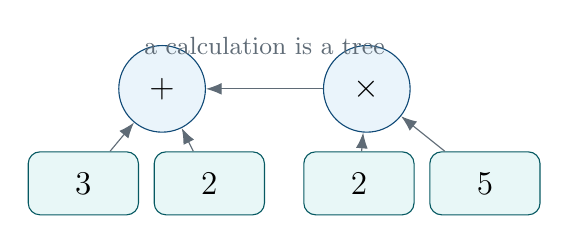
\begin{tikzpicture}[node distance=8mm, every node/.style={font=\large\bfseries,align=center},
  op/.style={circle,draw=blue!70!black,fill=bluepale,minimum size=11mm},
  leaf/.style={rounded corners=1.5mm,draw=teal!70!black,fill=tealpale,minimum width=14mm,minimum height=8mm},
  arr/.style={-{Latex[length=2mm]},draw=muted}]
  \node[op] (plus) at (0,0) {$+$};
  \node[op] (times) at (2.6,0) {$\times$};
  \node[leaf] (a) at (-1.0,-1.2) {$3$};
  \node[leaf] (b) at (0.6,-1.2) {$2$};
  \node[leaf] (c) at (2.5,-1.2) {$2$};
  \node[leaf] (d) at (4.1,-1.2) {$5$};
  \draw[arr] (a)--(plus); \draw[arr] (b)--(plus);
  \draw[arr] (c)--(times); \draw[arr] (d)--(times);
  \draw[arr] (times)--(plus);
  \node[font=\small,muted] at (1.3,0.55) {a calculation is a tree};
\end{tikzpicture}
\end{center}

\section{Fractions, ratios, and percentages}

A fraction $\frac{a}{b}$ is a quotient, a proportion, and a point on the number line. The denominator says how many equal parts make one whole; the numerator says how many parts we have. A ratio compares two quantities without necessarily making a whole: $2:3$ means that for every $2$ units of one thing there are $3$ units of another.

\begin{center}
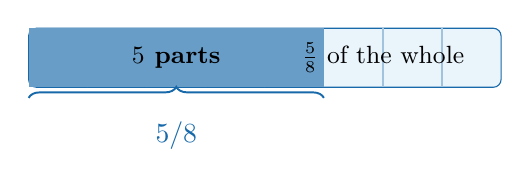
\begin{tikzpicture}[x=0.75cm,y=0.75cm]
  \draw[fill=bluepale,draw=blue,rounded corners=1mm] (0,0) rectangle (8,1);
  \foreach \x in {1,...,7}{\draw[blue!40] (\x,0)--(\x,1);}
  \foreach \x in {0,1,2,3,4}{\fill[blue!65] (\x,0) rectangle (\x+1,1);}
  \node[font=\small\bfseries] at (2.5,0.5) {$5$ parts};
  \node[font=\small] at (6,0.5) {$\frac{5}{8}$ of the whole};
  \draw[decorate,decoration={brace,amplitude=4pt},blue,line width=0.7pt] (0,-0.18)--(5,-0.18) node[midway,below=5pt] {$5/8$};
\end{tikzpicture}
\end{center}

The same relationship can be represented in several useful languages:
\[
  \frac{3}{4}=0.75=75\%=3:4.
\]
Percentages are ratios with denominator $100$. Proportional reasoning is the ability to move between these equivalent views without losing the meaning.

\section{Powers, roots, and logarithms}

An exponent records repeated multiplication: $a^3=a\cdot a\cdot a$. A root reverses a power: $\sqrt[3]{8}=2$. A logarithm asks for the exponent: $\log_2(8)=3$ because $2^3=8$.

\begin{center}
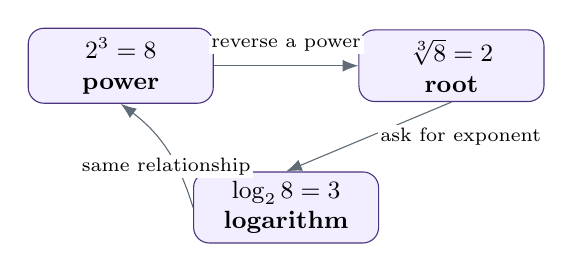
\begin{tikzpicture}[every node/.style={font=\small\bfseries},
  q/.style={rounded corners=2mm,draw=purple!70!black,fill=purplepale,minimum width=2.35cm,minimum height=0.8cm,align=center},
  arr/.style={-{Latex[length=2mm]},draw=muted}]
  \node[q] (pow) at (0,0) {$2^3=8$\\power};
  \node[q] (root) at (4.2,0) {$\sqrt[3]{8}=2$\\root};
  \node[q] (log) at (2.1,-1.8) {$\log_2 8=3$\\logarithm};
  \draw[arr] (pow.east)--node[above=4pt,font=\scriptsize,fill=white,inner sep=1pt]{reverse a power}(root.west);
  \draw[arr] (root.south)--node[right=3pt,font=\scriptsize,fill=white,inner sep=1pt]{ask for exponent}(log.north);
  \draw[arr] (log.west) to[bend right=18] node[below=2pt,font=\scriptsize,fill=white,inner sep=1pt]{same relationship} (pow.south);
\end{tikzpicture}
\end{center}

The laws $a^ma^n=a^{m+n}$ and $(a^m)^n=a^{mn}$ are not arbitrary rules. They express how repeated multiplication combines. Logarithms turn multiplication into addition:
\[
  \log(ab)=\log a+\log b,
  \qquad \log\left(\frac{a}{b}\right)=\log a-\log b.
\]

\section{Absolute value and distance}

The absolute value $\abs{x}$ is distance from zero, so it is never negative. More generally, $\abs{x-a}$ is the distance from $x$ to $a$. This gives a visual meaning to inequalities:
\[
  \abs{x-3}<2 \quad\Longleftrightarrow\quad 1<x<5.
\]

\begin{center}
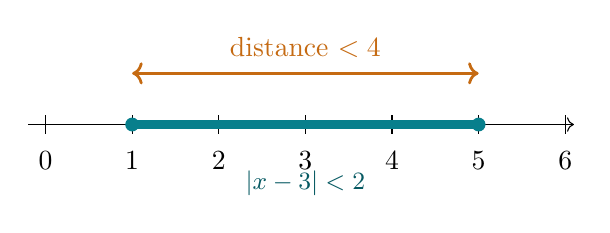
\begin{tikzpicture}[x=1.1cm]
  \draw[->] (-0.2,0)--(6.1,0);
  \foreach \x in {0,1,2,3,4,5,6}{\draw (\x,0.12)--(\x,-0.12) node[below=3pt] {\x};}
  \draw[teal,line width=3pt] (1,0)--(5,0);
  \fill[teal] (1,0) circle (2.5pt); \fill[teal] (5,0) circle (2.5pt);
  \draw[orange,line width=1pt,<->] (1,0.65)--(5,0.65) node[midway,above=2pt] {distance $<4$};
  \node[font=\small,teal!70!black] at (3,-0.75) {$\abs{x-3}<2$};
\end{tikzpicture}
\end{center}

\chapter{Algebra: relationships made visible}

\section{Variables are names for changing quantities}

A variable is not a mysterious letter. It is a placeholder whose value can vary. The expression $2x+3$ describes a process: start with $x$, double it, then add $3$. An equation says that two expressions have the same value.

\begin{center}
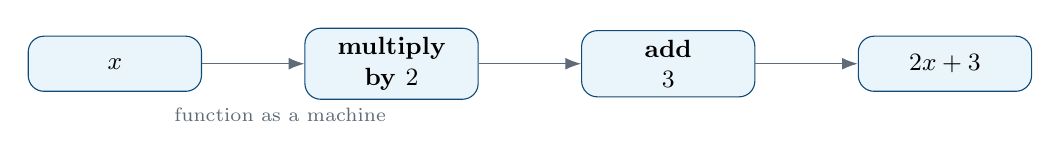
\begin{tikzpicture}[node distance=9mm and 13mm, every node/.style={font=\small\bfseries,align=center},
  p/.style={rounded corners=2mm,draw=blue!70!black,fill=bluepale,minimum width=2.2cm,minimum height=0.7cm},
  arr/.style={-{Latex[length=2mm]},draw=muted}]
  \node[p] (input) {$x$};
  \node[p,right=of input] (scale) {multiply\\by $2$};
  \node[p,right=of scale] (shift) {add\\$3$};
  \node[p,right=of shift] (output) {$2x+3$};
  \draw[arr] (input)--(scale); \draw[arr] (scale)--(shift); \draw[arr] (shift)--(output);
  \node[font=\scriptsize,muted] at (2.1,-0.65) {function as a machine};
\end{tikzpicture}
\end{center}

\begin{definition}
A function assigns exactly one output to each allowed input. We write $f(x)$ for the output associated with input $x$. The input set is the domain; the possible outputs form the range.
\end{definition}

\section{Solving equations means preserving balance}

An equation can be pictured as a balanced scale. Whatever operation we perform on one side must be performed on the other. To solve $3x+2=14$, subtract $2$ from both sides and divide both sides by $3$:
\[
  3x+2=14\quad\Longrightarrow\quad 3x=12\quad\Longrightarrow\quad x=4.
\]

\begin{center}
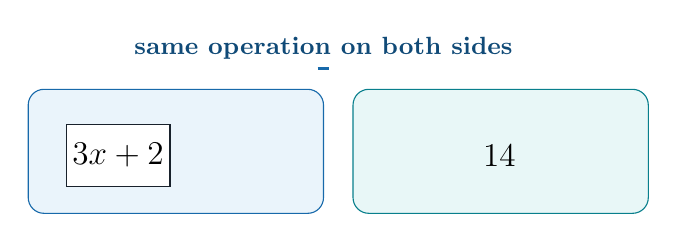
\begin{tikzpicture}[scale=0.75]
  \draw[fill=bluepale,draw=blue,rounded corners=2mm] (-5,0) rectangle (0,2.1);
  \draw[fill=tealpale,draw=teal,rounded corners=2mm] (0.5,0) rectangle (5.5,2.1);
  \draw[fill=white,draw=ink] (-4.35,0.45) rectangle (-2.6,1.5);
  \node[font=\large\bfseries] at (-3.48,0.98) {$3x+2$};
  \node[font=\large\bfseries] at (2.98,0.98) {$14$};
  \draw[blue,line width=1.2pt] (-0.1,2.45)--(0.1,2.45);
  \node[font=\small\bfseries,blue!70!black] at (0,2.8) {same operation on both sides};
\end{tikzpicture}
\end{center}

\begin{warningbox}{A common trap}
Dividing by an expression can lose solutions if that expression might be zero. For example, multiplying by $x$ is not reversible at $x=0$. Always record restrictions before cancelling.
\end{warningbox}

\section{Lines and slope}

The graph of $y=mx+b$ is a straight line. The intercept $b$ is the height where the line crosses the $y$-axis. The slope $m$ is rise over run:
\[
  m=\frac{\Delta y}{\Delta x}=\frac{y_2-y_1}{x_2-x_1}.
\]

\begin{center}
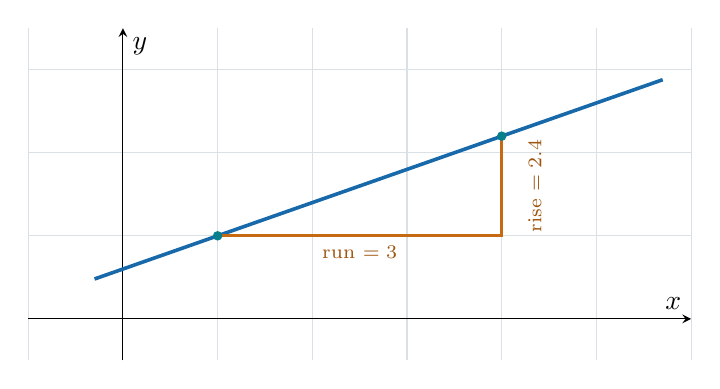
\begin{tikzpicture}
\begin{axis}[width=10cm,height=5.8cm,axis lines=middle,xmin=-1,xmax=6,ymin=-1,ymax=7,grid=both,major grid style={draw=linegray},xlabel={$x$},ylabel={$y$},ticks=none]
  \addplot[blue,line width=1.3pt,domain=-0.3:5.7]{0.8*x+1.2};
  \addplot[only marks,mark=*,mark size=1.5pt,teal] coordinates {(1,2) (4,4.4)};
  \draw[orange,line width=1pt] (1,2)--(4,2)--(4,4.4);
  \node[font=\scriptsize,orange!80!black] at (2.5,1.6) {run $=3$};
  \node[font=\scriptsize,orange!80!black,rotate=90] at (4.35,3.2) {rise $=2.4$};
\end{axis}
\end{tikzpicture}
\end{center}

Slope is a local rate: how much output changes for one unit of input. This idea becomes the derivative in calculus.

\section{Quadratics and factorisation}

A quadratic has the form $ax^2+bx+c$. Its graph is a parabola. Factoring rewrites a product hidden inside a sum:
\[
  x^2-5x+6=(x-2)(x-3).
\]
The roots are where the graph touches or crosses the horizontal axis. The quadratic formula solves every quadratic with $a\ne0$:
\[
  x=\frac{-b\pm\sqrt{b^2-4ac}}{2a}.
\]
The discriminant $\Delta=b^2-4ac$ tells the geometry: $\Delta>0$ gives two real roots, $\Delta=0$ gives one repeated root, and $\Delta<0$ gives no real roots.

\begin{center}
\begin{tikzpicture}[x=1.1cm,y=0.6cm]
  \draw[->] (-3.6,0)--(4.2,0) node[right] {$x$};
  \draw[->] (0,-1.1)--(0,6.4) node[above] {$y$};
  \draw[blue,line width=1.3pt,samples=100,domain=-2.1:3.2] plot (\x,{0.75*(\x-2)*(\x-2)-0.5});
  \fill[teal] (2,-0.5) circle (2.4pt) node[below right,font=\small] {vertex};
  \fill[orange] (1.184,0) circle (2.3pt); \fill[orange] (2.816,0) circle (2.3pt);
  \node[font=\small,orange!80!black] at (2,0.55) {roots};
\end{tikzpicture}
\end{center}

\section{Systems of equations}

Two equations in two unknowns describe two constraints. Their solution is a point satisfying both. Graphically, it is an intersection. Algebraically, elimination combines equations so that one variable disappears.

\begin{center}
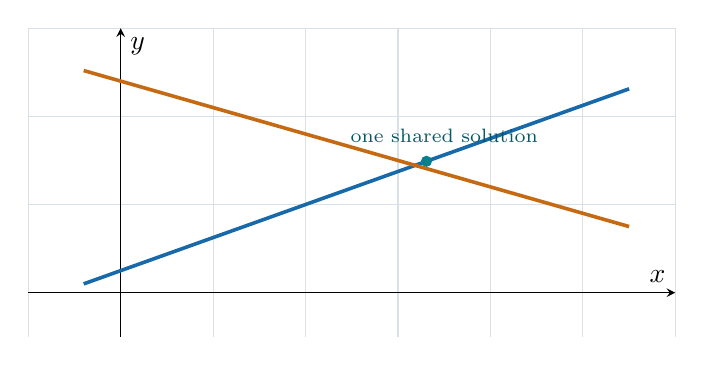
\begin{tikzpicture}
\begin{axis}[width=9.8cm,height=5.5cm,axis lines=middle,xmin=-1,xmax=6,ymin=-1,ymax=6,grid=both,major grid style={draw=linegray},ticks=none,xlabel={$x$},ylabel={$y$}]
  \addplot[blue,line width=1.3pt,domain=-0.4:5.5]{0.75*x+0.5};
  \addplot[orange,line width=1.3pt,domain=-0.4:5.5]{-0.6*x+4.8};
  \addplot[only marks,mark=*,mark size=1.8pt,teal] coordinates {(3.3077,2.9808)};
  \node[font=\scriptsize,teal!70!black] at (3.5,3.55) {one shared solution};
\end{axis}
\end{tikzpicture}
\end{center}

\section{Functions as shapes}

Changing a formula changes the graph in systematic ways. If $y=f(x)$, then $f(x)+k$ shifts the graph vertically, $f(x-h)$ shifts it right by $h$, $-f(x)$ reflects it across the $x$-axis, and $f(-x)$ reflects it across the $y$-axis.

\begin{center}
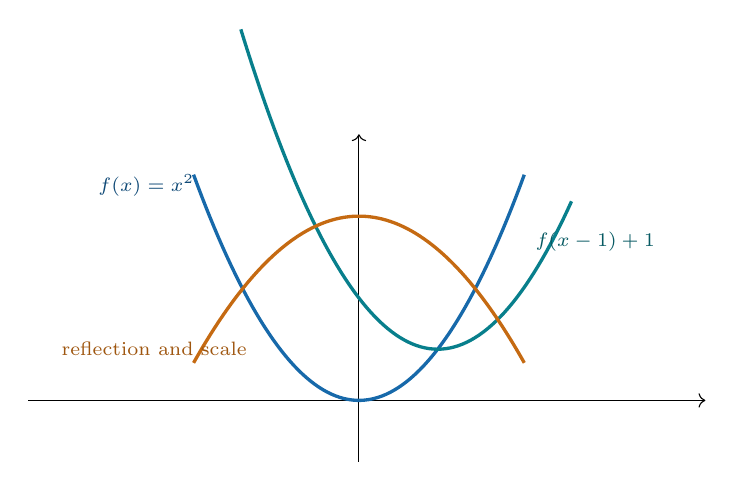
\begin{tikzpicture}[x=1cm,y=0.65cm]
  \draw[->] (-4.2,0)--(4.4,0); \draw[->] (0,-1.2)--(0,5.2);
  \draw[blue,line width=1.2pt,samples=80,domain=-2.1:2.1] plot (\x,{\x*\x});
  \draw[teal,line width=1.2pt,samples=80,domain=-1.5:2.7] plot (\x,{(\x-1)* (\x-1)+1});
  \draw[orange,line width=1.2pt,samples=80,domain=-2.1:2.1] plot (\x,{-0.65*\x*\x+3.6});
  \node[font=\scriptsize,blue!70!black] at (-2.7,4.2) {$f(x)=x^2$};
  \node[font=\scriptsize,teal!70!black] at (3.0,3.1) {$f(x-1)+1$};
  \node[font=\scriptsize,orange!80!black] at (-2.6,1.0) {reflection and scale};
\end{tikzpicture}
\end{center}

\chapter{Geometry and trigonometry}

\section{Shape is measurement with structure}

Geometry studies points, lines, angles, curves, surfaces, and solids. A measurement becomes meaningful when the relationships between parts are known. Similar figures have the same angles and proportional side lengths; congruent figures have the same shape and size.

\begin{center}
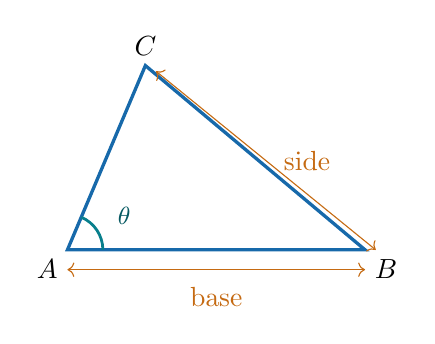
\begin{tikzpicture}[scale=0.9]
  \coordinate (A) at (0,0); \coordinate (B) at (4.2,0); \coordinate (C) at (1.1,2.6);
  \draw[blue,line width=1.2pt] (A)--(B)--(C)--cycle;
  \draw[teal,line width=1.0pt] (A) ++(0.5,0) arc (0:67:0.5);
  \node[below left] at (A) {$A$}; \node[below right] at (B) {$B$}; \node[above] at (C) {$C$};
  \node[font=\small,teal!70!black] at (0.8,0.48) {$\theta$};
  \draw[orange,<->] (0,-0.28)--(4.2,-0.28) node[midway,below=3pt] {base};
  \draw[orange,<->] (4.35,0)--(1.25,2.52) node[midway,right=3pt] {side};
\end{tikzpicture}
\end{center}

\section{Similarity and the Pythagorean theorem}

Right triangles connect length to angle. If the legs are $a$ and $b$ and the hypotenuse is $c$, then
\[
  a^2+b^2=c^2.
\]
The theorem is not only a formula for missing sides. It says that the square built on the hypotenuse has exactly the same area as the two squares built on the legs.

\begin{center}
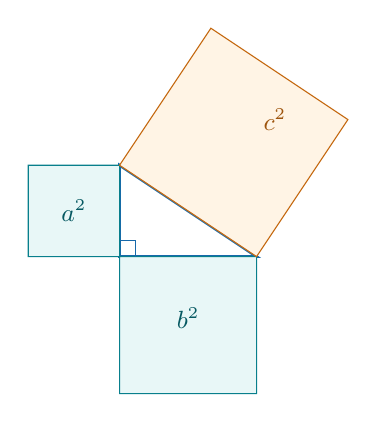
\begin{tikzpicture}[scale=0.58]
  \coordinate (A) at (0,0); \coordinate (B) at (3,0); \coordinate (C) at (0,2);
  \draw[blue,line width=1pt] (A)--(B)--(C)--cycle;
  \draw[teal,fill=tealpale] (A)--(C)--(-2,2)--(-2,0)--cycle;
  \draw[teal,fill=tealpale] (A)--(B)--(3,-3)--(0,-3)--cycle;
  \draw[orange,fill=orangepale] (B)--(C)--(2,5)--(5,3)--cycle;
  \node[font=\small\bfseries,teal!70!black] at (-1.0,1.0) {$a^2$};
  \node[font=\small\bfseries,teal!70!black] at (1.5,-1.35) {$b^2$};
  \node[font=\small\bfseries,orange!80!black] at (3.4,3.0) {$c^2$};
  \draw[blue] (0.35,0) -- (0.35,0.35) -- (0,0.35);
\end{tikzpicture}
\end{center}

\section{The circle and radian measure}

The circumference of a circle is $2\pi r$, and its area is $\pi r^2$. An angle measured in radians is the arc length divided by the radius. A full turn is $2\pi$ radians, a half turn is $\pi$, and a right angle is $\pi/2$.

\begin{center}
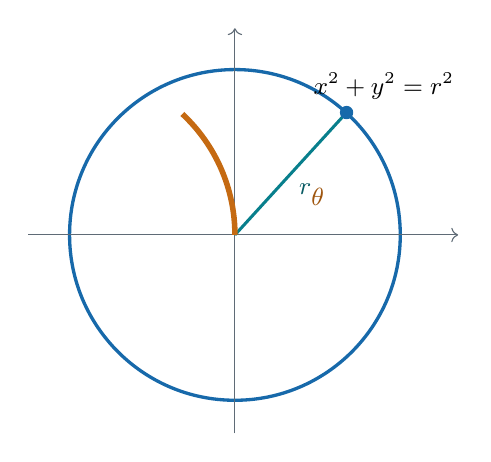
\begin{tikzpicture}[scale=1.05]
  \draw[blue,line width=1.2pt] (0,0) circle (2);
  \draw[->,muted] (-2.5,0)--(2.7,0); \draw[->,muted] (0,-2.4)--(0,2.5);
  \coordinate (P) at (1.35,1.48);
  \draw[teal,line width=1.1pt] (0,0)--(P);
  \draw[orange,line width=2pt] (0,0) arc (0:47:2);
  \node[font=\small,teal!70!black] at (0.85,0.55) {$r$};
  \node[font=\small,orange!80!black] at (1.0,0.46) {$\theta$};
  \fill[blue] (P) circle (2.3pt);
  \node[font=\small] at (1.8,1.8) {$x^2+y^2=r^2$};
\end{tikzpicture}
\end{center}

\section{Sine, cosine, and tangent}

For a point on the unit circle at angle $\theta$, the coordinates are $(\cos\theta,\sin\theta)$. This single picture explains periodic motion, right-triangle ratios, and the graphs of trigonometric functions.

\begin{center}
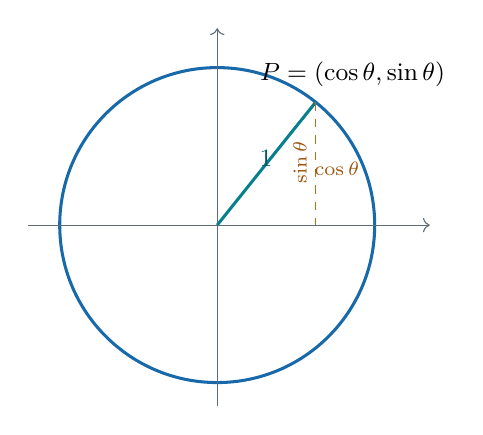
\begin{tikzpicture}[x=1.0cm,y=1.0cm]
  \draw[blue,line width=1.1pt] (0,0) circle (2);
  \draw[->,muted] (-2.4,0)--(2.7,0); \draw[->,muted] (0,-2.3)--(0,2.5);
  \coordinate (P) at (1.25,1.56);
  \draw[teal,line width=1.1pt] (0,0)--(P);
  \draw[orange,dashed] (P)--(1.25,0);
  \node[font=\small,teal!70!black] at (0.62,0.85) {$1$};
  \node[font=\scriptsize,orange!80!black] at (1.52,0.72) {$\cos\theta$};
  \node[font=\scriptsize,orange!80!black,rotate=90] at (1.05,0.8) {$\sin\theta$};
  \node[font=\small] at (1.72,1.92) {$P=(\cos\theta,\sin\theta)$};
\end{tikzpicture}
\end{center}

\[
  \sin^2\theta+\cos^2\theta=1,
  \qquad \tan\theta=\frac{\sin\theta}{\cos\theta}.
\]
The identities are geometric consequences of the unit circle, not isolated facts to memorise.

\section{Vectors and coordinates}

A vector has magnitude and direction. In the plane, $\vect v=(v_x,v_y)$. Its length is
\[
  \norm{\vect v}=\sqrt{v_x^2+v_y^2}.
\]
Adding vectors is head-to-tail movement. Multiplying a vector by a scalar changes its length and possibly reverses its direction.

\begin{center}
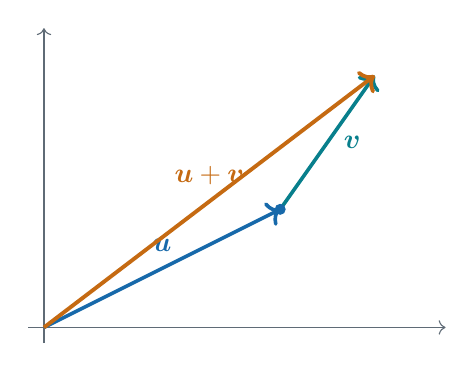
\begin{tikzpicture}[x=1cm,y=1cm]
  \draw[->,muted] (-0.2,0)--(5.1,0); \draw[->,muted] (0,-0.2)--(0,3.8);
  \draw[->,blue,line width=1.3pt] (0,0)--(3,1.5) node[midway,above=2pt] {$\vect u$};
  \draw[->,teal,line width=1.3pt] (3,1.5)--(4.2,3.2) node[midway,right=2pt] {$\vect v$};
  \draw[->,orange,line width=1.4pt] (0,0)--(4.2,3.2) node[midway,above=2pt] {$\vect u+\vect v$};
  \fill[blue] (3,1.5) circle (2pt);
\end{tikzpicture}
\end{center}

\chapter{Coordinates and functions}

\section{The plane is a relationship between two numbers}

An ordered pair $(x,y)$ is a location: move $x$ units horizontally and $y$ vertically. A curve is a set of points obeying a rule. The equation $x^2+y^2=1$ describes every point one unit from the origin.

\begin{center}
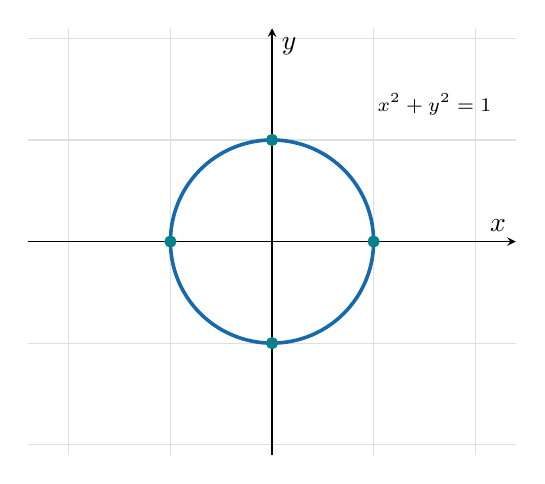
\begin{tikzpicture}
\begin{axis}[width=9.4cm,height=7cm,axis equal image,axis lines=middle,xmin=-2.4,xmax=2.4,ymin=-2.1,ymax=2.1,grid=both,major grid style={draw=linegray},xlabel={$x$},ylabel={$y$},ticks=none]
  \addplot[blue,line width=1.3pt,domain=0:360,samples=160] ({cos(x)},{sin(x)});
  \addplot[only marks,mark=*,teal] coordinates {(1,0) (0,1) (-1,0) (0,-1)};
  \node[font=\scriptsize] at (1.6,1.35) {$x^2+y^2=1$};
\end{axis}
\end{tikzpicture}
\end{center}

\section{Domain, range, and inverse functions}

The domain asks, ``what inputs are allowed?'' The range asks, ``what outputs can occur?'' For $f(x)=\sqrt{x-2}$, the domain is $x\ge2$ and the range is $y\ge0$. An inverse function reverses the input-output process. If $f$ maps $x$ to $y$, then $f^{-1}$ maps $y$ back to $x$, provided the original function does not send two different inputs to the same output.

\begin{center}
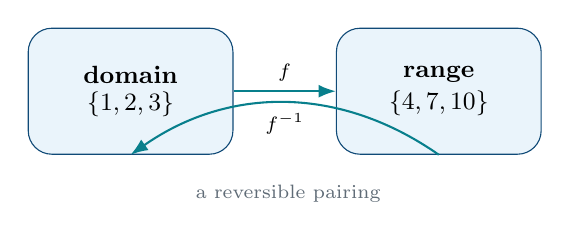
\begin{tikzpicture}[node distance=13mm, every node/.style={font=\small\bfseries},
  set/.style={rounded corners=3mm,draw=blue!70!black,fill=bluepale,minimum width=2.6cm,minimum height=1.6cm},
  arr/.style={-{Latex[length=2.2mm]},draw=teal,line width=0.75pt}]
  \node[set] (dom) {\shortstack{domain\\$\{1,2,3\}$}};
  \node[set,right=of dom] (ran) {\shortstack{range\\$\{4,7,10\}$}};
  \draw[arr] (dom.east)--node[above,font=\scriptsize] {$f$}(ran.west);
  \draw[arr] (ran.south) to[bend right=35] node[below,font=\scriptsize] {$f^{-1}$} (dom.south);
  \node[font=\scriptsize,muted] at (2.0,-1.3) {a reversible pairing};
\end{tikzpicture}
\end{center}

\section{Exponential growth and decay}

The function $f(t)=Ae^{kt}$ models proportional change: the rate of change is always a fixed fraction $k$ of the current amount. If $k>0$, the graph grows; if $k<0$, it decays. Doubling time and half-life are logarithmic questions.

\begin{center}
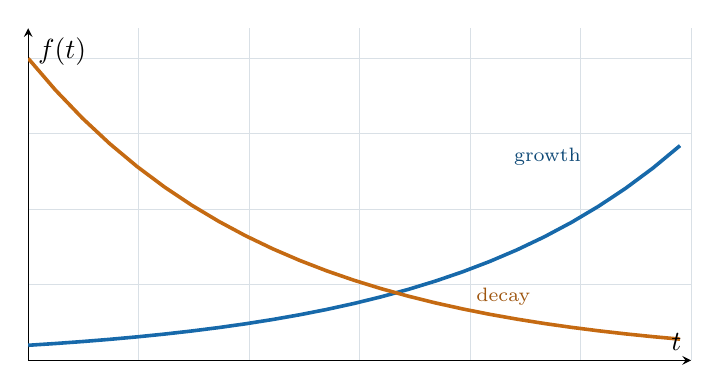
\begin{tikzpicture}
\begin{axis}[width=10cm,height=5.8cm,axis lines=middle,xmin=0,xmax=6,ymin=0,ymax=22,grid=both,major grid style={draw=linegray},xlabel={$t$},ylabel={$f(t)$},ticks=none]
  \addplot[blue,line width=1.3pt,domain=0:5.9]{exp(0.45*x)};
  \addplot[orange,line width=1.3pt,domain=0:5.9]{20*exp(-0.45*x)};
  \node[font=\scriptsize,blue!70!black] at (4.7,13.5) {growth};
  \node[font=\scriptsize,orange!80!black] at (4.3,4.2) {decay};
\end{axis}
\end{tikzpicture}
\end{center}

\section{Sequences and series}

A sequence is an ordered list. An arithmetic sequence adds the same amount each time; a geometric sequence multiplies by the same factor. A series adds the terms of a sequence. The finite geometric sum is
\[
  1+r+r^2+\cdots+r^n=\frac{1-r^{n+1}}{1-r},\qquad r\ne1.
\]
When $\abs r<1$, the infinite series approaches the limit $1/(1-r)$. The visual idea is repeated shrinking: each new piece is a fixed fraction of the previous piece.

\begin{center}
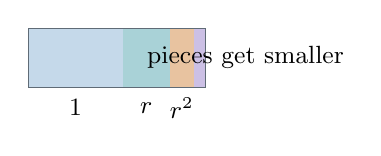
\begin{tikzpicture}[x=1.2cm,y=0.75cm]
  \fill[blue!25] (0,0) rectangle (1,1);
  \fill[teal!35] (1,0) rectangle (1.5,1);
  \fill[orange!40] (1.5,0) rectangle (1.75,1);
  \fill[purple!35] (1.75,0) rectangle (1.875,1);
  \draw[muted] (0,0) rectangle (1.875,1);
  \node[font=\small] at (0.5,-0.35) {$1$};
  \node[font=\small] at (1.25,-0.35) {$r$};
  \node[font=\small] at (1.625,-0.35) {$r^2$};
  \node[font=\small] at (2.3,0.5) {pieces get smaller};
\end{tikzpicture}
\end{center}

\chapter{Limits and calculus}

\section{A limit is a destination}

A limit describes what a quantity approaches, even if it never arrives. Write
\[
  \lim_{x\to a}f(x)=L
\]
when the values of $f(x)$ get arbitrarily close to $L$ as $x$ gets close to $a$. This lets us define instantaneous change from average change.

\begin{center}
\begin{tikzpicture}[x=1.2cm,y=0.72cm]
  \draw[->] (-2.6,0)--(2.8,0) node[right] {$x$};
  \draw[->] (0,-0.5)--(0,4.8) node[above] {$f(x)$};
  \draw[blue,line width=1.2pt,samples=100,domain=-2.1:2.1] plot (\x,{0.45*\x*\x+1.1});
  \draw[orange,dashed] (1.3,0)--(1.3,1.86); \draw[orange,dashed] (0,1.86)--(1.3,1.86);
  \fill[teal] (1.3,1.86) circle (2.3pt);
  \node[font=\small,orange!80!black] at (1.3,-0.35) {$a$};
  \node[font=\small,teal!70!black] at (0.62,2.14) {$L$};
\end{tikzpicture}
\end{center}

\section{The derivative is local slope}

The average slope between two points is
\[
  \frac{f(x+h)-f(x)}{h}.
\]
Letting $h$ shrink toward zero gives the derivative:
\[
  f'(x)=\lim_{h\to0}\frac{f(x+h)-f(x)}{h}.
\]
It is the slope of the tangent line, the instantaneous rate of change, and the best linear approximation at a point.

\begin{center}
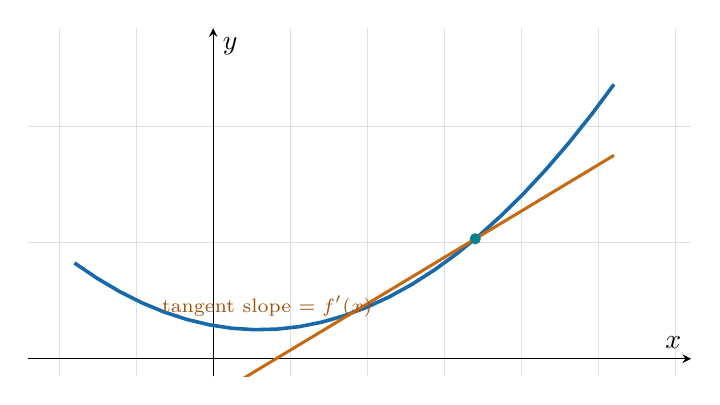
\begin{tikzpicture}
\begin{axis}[width=10cm,height=6cm,axis lines=middle,xmin=-1.2,xmax=3.1,ymin=-0.3,ymax=5.7,grid=both,major grid style={draw=linegray},ticks=none,xlabel={$x$},ylabel={$y$}]
  \addplot[blue,line width=1.3pt,domain=-0.9:2.6]{0.8*(x-0.3)^2+0.5};
  \addplot[orange,line width=1.1pt,domain=-0.9:2.6]{1.6*(x-1.7)+2.068};
  \addplot[only marks,mark=*,teal,mark size=1.8pt] coordinates {(1.7,2.068)};
  \node[font=\scriptsize,orange!80!black] at (0.35,0.9) {tangent slope $=f'(x)$};
\end{axis}
\end{tikzpicture}
\end{center}

The power rule follows from the definition:
\[
  \frac{\dd}{\dd x}x^n=nx^{n-1}.
\]
The product rule, quotient rule, and chain rule are bookkeeping rules for how changes combine:
\[
  (fg)'=f'g+fg',\qquad (f\circ g)'(x)=f'(g(x))g'(x).
\]

\section{Optimisation and the shape of a graph}

At a smooth local maximum or minimum, the tangent is horizontal, so $f'(x)=0$. This is a candidate, not a guarantee. The second derivative tells how the slope itself is changing: $f''(x)>0$ means the graph bends upward locally; $f''(x)<0$ means it bends downward.

\begin{center}
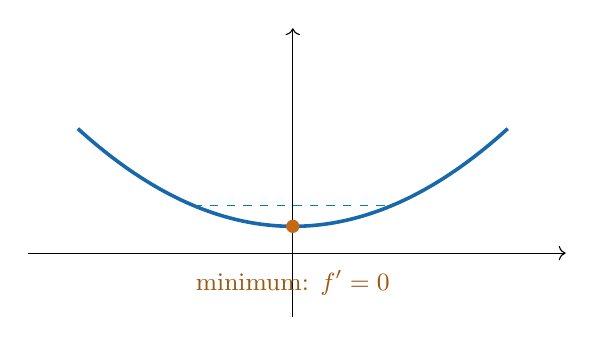
\begin{tikzpicture}[x=1.05cm,y=0.68cm]
  \draw[->] (-3.2,0)--(3.3,0); \draw[->] (0,-1.2)--(0,4.2);
  \draw[blue,line width=1.3pt,samples=100,domain=-2.6:2.6] plot (\x,{0.27*\x*\x+0.5});
  \draw[teal,dashed] (-1.2,0.89)--(1.2,0.89);
  \fill[orange] (0,0.5) circle (2.4pt);
  \node[font=\small,orange!80!black] at (0,-0.55) {minimum: $f'=0$};
\end{tikzpicture}
\end{center}

\section{The integral is accumulation}

The definite integral adds infinitely many thin slices. Geometrically, it is signed area under a curve; physically, it can be accumulated distance from velocity or total mass from density.

\begin{center}
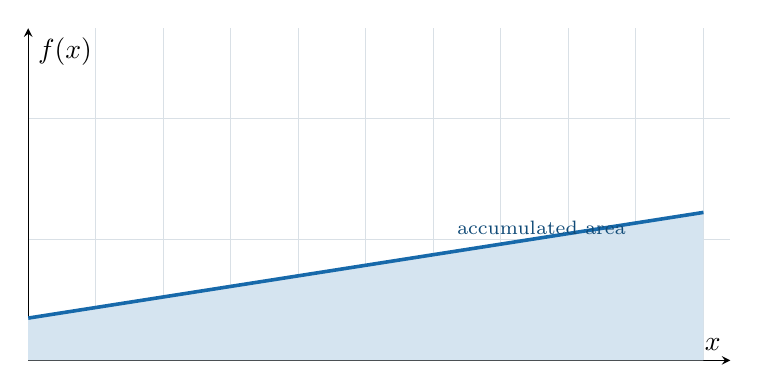
\begin{tikzpicture}
\begin{axis}[width=10.5cm,height=5.8cm,axis lines=middle,xmin=0,xmax=5.2,ymin=0,ymax=5.5,grid=both,major grid style={draw=linegray},ticks=none,xlabel={$x$},ylabel={$f(x)$}]
  \addplot[name path=curve,blue,line width=1.3pt,domain=0:5]{0.35*x+0.7};
  \path[name path=axis] (axis cs:0,0)--(axis cs:5,0);
  \addplot[blue!18] fill between[of=curve and axis,soft clip={domain=0:5}];
  \node[font=\scriptsize,blue!70!black] at (3.8,2.2) {accumulated area};
\end{axis}
\end{tikzpicture}
\end{center}

The fundamental theorem of calculus connects the two central operations:
\[
  \int_a^b f(x)\dd x=F(b)-F(a)\quad\text{when }F'(x)=f(x).
\]
Differentiation measures local change; integration rebuilds total change.

\section{Multivariable calculus}

For $f(x,y)$, the surface height depends on two inputs. A partial derivative changes one coordinate while holding the other fixed. The gradient
\[
  \nabla f=\left(\frac{\partial f}{\partial x},\frac{\partial f}{\partial y}\right)
\]
points in the direction of steepest increase. Level curves $f(x,y)=c$ are contour lines; the gradient is perpendicular to them.

\begin{center}
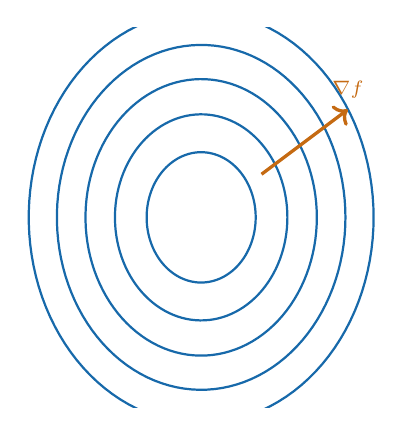
\begin{tikzpicture}
\begin{axis}[view={0}{90},width=10.5cm,height=6.4cm,axis equal image,xmin=-2.2,xmax=2.2,ymin=-2.2,ymax=2.2,axis lines=none,ticks=none]
  \addplot[blue,line width=0.8pt,domain=0:360,samples=120] ({sqrt(0.4)*cos(x)},{sqrt(0.4/0.7)*sin(x)});
  \addplot[blue,line width=0.8pt,domain=0:360,samples=120] ({sqrt(1)*cos(x)},{sqrt(1/0.7)*sin(x)});
  \addplot[blue,line width=0.8pt,domain=0:360,samples=120] ({sqrt(1.8)*cos(x)},{sqrt(1.8/0.7)*sin(x)});
  \addplot[blue,line width=0.8pt,domain=0:360,samples=120] ({sqrt(2.8)*cos(x)},{sqrt(2.8/0.7)*sin(x)});
  \addplot[blue,line width=0.8pt,domain=0:360,samples=120] ({sqrt(4)*cos(x)},{sqrt(4/0.7)*sin(x)});
  \draw[->,orange,line width=1.2pt] (axis cs:0.7,0.5)--(axis cs:1.7,1.25) node[above,font=\scriptsize] {$\nabla f$};
\end{axis}
\end{tikzpicture}
\end{center}

\chapter{Linear algebra: vectors, matrices, and maps}

\section{Vectors are directed quantities}

Vectors can represent position, velocity, force, data features, or directions in an abstract space. A vector space is a collection where vectors can be added and scaled while following consistent rules.

\begin{definition}
The dot product of $\vect u=(u_1,\ldots,u_n)$ and $\vect v=(v_1,\ldots,v_n)$ is
\[
  \vect u\cdot\vect v=\sum_{i=1}^n u_iv_i.
\]
It measures alignment: $\vect u\cdot\vect v=0$ means perpendicular, positive means broadly pointing together, and negative means broadly opposing.
\end{definition}

\begin{center}
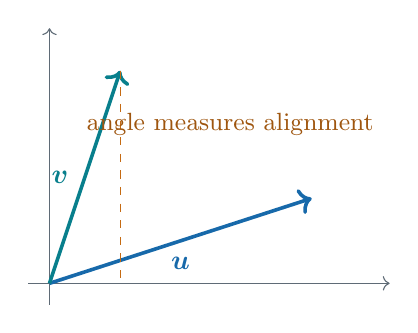
\begin{tikzpicture}[x=0.9cm,y=0.9cm]
  \draw[->,muted] (-0.3,0)--(4.8,0); \draw[->,muted] (0,-0.3)--(0,3.6);
  \draw[->,blue,line width=1.3pt] (0,0)--(3.7,1.2) node[midway,below=2pt] {$\vect u$};
  \draw[->,teal,line width=1.3pt] (0,0)--(1.0,3.0) node[midway,left=2pt] {$\vect v$};
  \draw[orange,dashed] (1.0,3.0)--(1.0,0);
  \node[font=\small,orange!80!black] at (2.55,2.25) {angle measures alignment};
\end{tikzpicture}
\end{center}

\section{Matrices are machines for vectors}

A matrix is a rectangular array of numbers, but its most important meaning is as a function that maps vectors to vectors. Matrix multiplication composes transformations.

\begin{center}
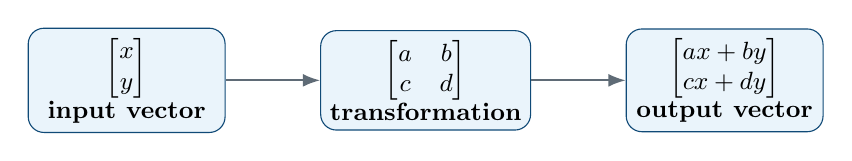
\begin{tikzpicture}[node distance=12mm, every node/.style={font=\small\bfseries,align=center},
  mat/.style={rounded corners=2mm,draw=blue!70!black,fill=bluepale,minimum width=2.5cm,minimum height=1.0cm},
  arr/.style={-{Latex[length=2.2mm]},draw=muted,line width=0.7pt}]
  \node[mat] (v) {$\begin{bmatrix}x\\y\end{bmatrix}$\\input vector};
  \node[mat,right=of v] (m) {$\begin{bmatrix}a&b\\c&d\end{bmatrix}$\\transformation};
  \node[mat,right=of m] (out) {$\begin{bmatrix}ax+by\\cx+dy\end{bmatrix}$\\output vector};
  \draw[arr] (v)--(m); \draw[arr] (m)--(out);
\end{tikzpicture}
\end{center}

\begin{center}
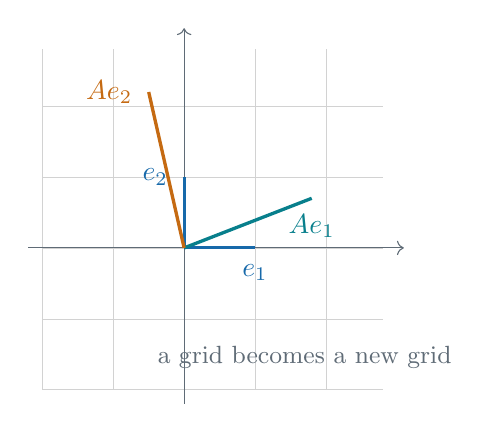
\begin{tikzpicture}[scale=0.9]
  \draw[step=1cm,gray!35,very thin] (-2,-2) grid (2.8,2.8);
  \draw[->,muted] (-2.2,0)--(3.1,0); \draw[->,muted] (0,-2.2)--(0,3.1);
  \draw[blue,line width=1.1pt] (0,0)--(1,0) node[below=2pt] {$e_1$};
  \draw[blue,line width=1.1pt] (0,0)--(0,1) node[left=2pt] {$e_2$};
  \draw[teal,line width=1.2pt] (0,0)--(1.8,0.7) node[below=2pt] {$Ae_1$};
  \draw[orange,line width=1.2pt] (0,0)--(-0.5,2.2) node[left=2pt] {$Ae_2$};
  \node[font=\small,muted] at (1.7,-1.55) {a grid becomes a new grid};
\end{tikzpicture}
\end{center}

The columns of a matrix are where the standard basis vectors go. That is why a matrix is determined by its action on the basis.

\section{Systems and elimination}

The system $A\vect x=\vect b$ asks for the input vector that the linear transformation $A$ sends to $\vect b$. Gaussian elimination changes the system into an easier but equivalent form by combining equations.

\begin{center}
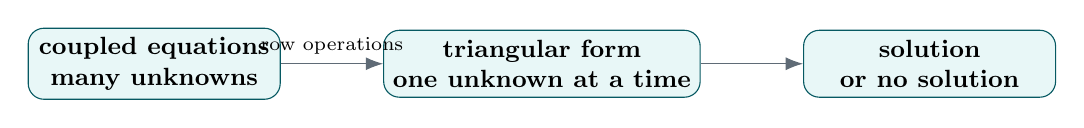
\begin{tikzpicture}[node distance=13mm, every node/.style={font=\small\bfseries,align=center},
  s/.style={rounded corners=2mm,draw=teal!70!black,fill=tealpale,minimum width=3.2cm,minimum height=0.85cm},
  a/.style={-{Latex[length=2.2mm]},draw=muted}]
  \node[s] (start) {coupled equations\\many unknowns};
  \node[s,right=of start] (tri) {triangular form\\one unknown at a time};
  \node[s,right=of tri] (sol) {solution\\or no solution};
  \draw[a] (start)--node[above,font=\scriptsize] {row operations}(tri);
  \draw[a] (tri)--(sol);
\end{tikzpicture}
\end{center}

\section{Determinants and eigenvectors}

The determinant of a square matrix measures signed area or volume scaling. If $\det(A)=0$, the transformation flattens space and cannot be inverted. An eigenvector is a direction that a transformation leaves unchanged except for scaling:
\[
  A\vect v=\lambda\vect v.
\]
Eigenvalues reveal stable directions, growth rates, oscillations, and long-run behaviour. They appear in differential equations, Markov chains, data compression, and quantum mechanics.

\begin{center}
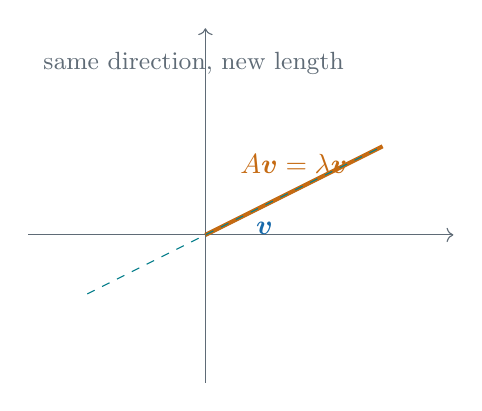
\begin{tikzpicture}[scale=0.75]
  \draw[->,muted] (-3,0)--(4.2,0); \draw[->,muted] (0,-2.5)--(0,3.5);
  \draw[blue,line width=1.2pt] (0,0)--(2,1) node[midway,below=2pt] {$\vect v$};
  \draw[orange,line width=1.5pt] (0,0)--(3,1.5) node[midway,above=2pt] {$A\vect v=\lambda\vect v$};
  \draw[teal,dashed] (-2,-1)--(3,1.5);
  \node[font=\small,muted] at (-0.2,2.9) {same direction, new length};
\end{tikzpicture}
\end{center}

\chapter{Probability and uncertainty}

\section{Outcomes, events, and sample spaces}

Probability begins by naming the possible outcomes. The sample space $\Omega$ is the set of all outcomes. An event $A$ is a subset of outcomes. A probability assigns a number from $0$ to $1$ to each event.

\begin{center}
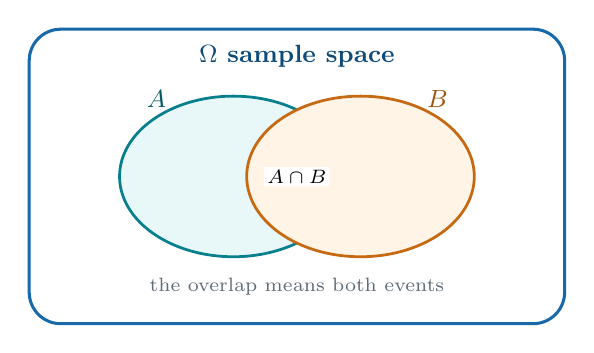
\begin{tikzpicture}[scale=0.85]
  \draw[blue,line width=1.1pt,rounded corners=4mm] (-4,-2.2) rectangle (4,2.2);
  \node[font=\small\bfseries,blue!70!black] at (0,1.8) {$\Omega$ sample space};
  \draw[fill=tealpale,draw=teal,line width=1pt] (-0.95,0) ellipse (1.7 and 1.2);
  \node[font=\small\bfseries,teal!70!black] at (-2.1,1.15) {$A$};
  \draw[fill=orangepale,draw=orange,line width=1pt] (0.95,0) ellipse (1.7 and 1.2);
  \node[font=\small\bfseries,orange!80!black] at (2.1,1.15) {$B$};
  \node[font=\scriptsize,fill=white,inner sep=1pt] at (0,0) {$A\cap B$};
  \node[font=\scriptsize,muted] at (0,-1.65) {the overlap means both events};
\end{tikzpicture}
\end{center}

The core rules are
\[
  P(\Omega)=1,\qquad P(A^c)=1-P(A),
\]
and for disjoint events $A$ and $B$,
\[
  P(A\cup B)=P(A)+P(B).
\]
For overlapping events, subtract the double count:
\[
  P(A\cup B)=P(A)+P(B)-P(A\cap B).
\]

\section{Conditional probability and Bayes' rule}

Conditional probability narrows the sample space. Given that $B$ happened, the probability of $A$ is
\[
  P(A\mid B)=\frac{P(A\cap B)}{P(B)}.
\]
Bayes' rule reverses the direction of conditioning:
\[
  P(A\mid B)=\frac{P(B\mid A)P(A)}{P(B)}.
\]

\begin{center}
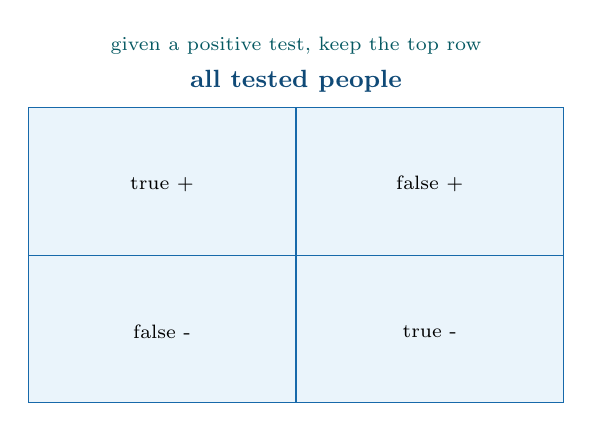
\begin{tikzpicture}[x=0.85cm,y=0.75cm]
  \draw[fill=bluepale,draw=blue] (0,0) rectangle (8,5);
  \draw[blue] (0,2.5)--(8,2.5); \draw[blue] (4,0)--(4,5);
  \node[font=\scriptsize] at (2,3.7) {true +};
  \node[font=\scriptsize] at (6,3.7) {false +};
  \node[font=\scriptsize] at (2,1.2) {false -};
  \node[font=\scriptsize] at (6,1.2) {true -};
  \node[font=\small\bfseries,blue!70!black] at (4,5.45) {all tested people};
  \node[font=\scriptsize,teal!70!black] at (4,6.05) {given a positive test, keep the top row};
\end{tikzpicture}
\end{center}

The key lesson is that a test's accuracy is not the same as the probability that a person with a positive result truly has the condition. Base rates matter.

\section{Random variables and distributions}

A random variable assigns a number to each outcome. Its distribution records how probability is spread across possible values. The expected value is a probability-weighted average:
\[
  \mathbb{E}[X]=\sum_x xP(X=x)
  \quad\text{or}\quad
  \mathbb{E}[X]=\int_{-\infty}^{\infty}x f_X(x)\dd x.
\]
Variance measures spread around the mean:
\[
  \operatorname{Var}(X)=\mathbb{E}\big[(X-\mathbb{E}X)^2\big].
\]

\begin{center}
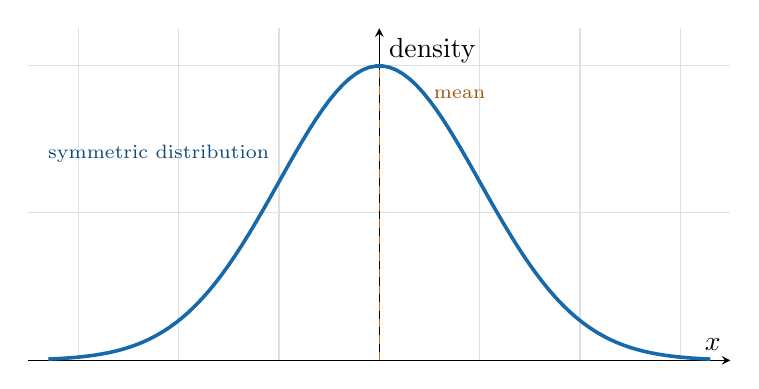
\begin{tikzpicture}
\begin{axis}[width=10.5cm,height=5.8cm,axis lines=middle,xmin=-3.5,xmax=3.5,ymin=0,ymax=0.45,grid=both,major grid style={draw=linegray},ticks=none,xlabel={$x$},ylabel={density}]
  \addplot[blue,line width=1.3pt,domain=-3.3:3.3,samples=100]{1/sqrt(2*pi)*exp(-x^2/2)};
  \draw[orange,dashed] (axis cs:0,0)--(axis cs:0,0.4);
  \node[font=\scriptsize,orange!80!black] at (axis cs:0.8,0.36) {mean};
  \node[font=\scriptsize,blue!70!black] at (axis cs:-2.2,0.28) {symmetric distribution};
\end{axis}
\end{tikzpicture}
\end{center}

\section{Independence and the law of large numbers}

Events $A$ and $B$ are independent when knowing one does not change the probability of the other:
\[
  P(A\cap B)=P(A)P(B).
\]
Independence is an assumption about the process, not a synonym for ``unrelated'' in everyday language. The law of large numbers says that averages of repeated independent observations tend to stabilise near the expected value.

\begin{center}
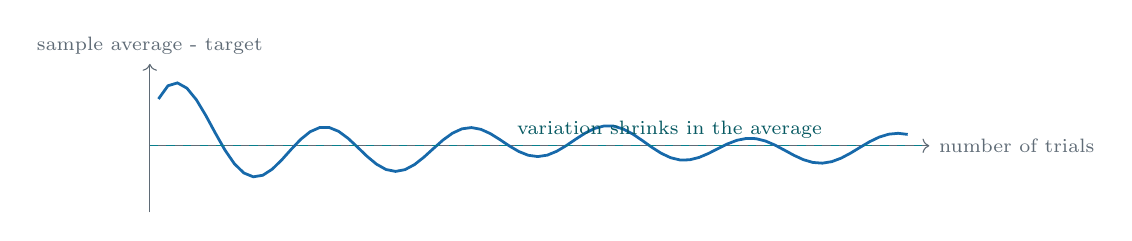
\begin{tikzpicture}[x=0.55cm,y=0.65cm]
  \draw[->,muted] (0,0)--(18,0) node[right,font=\scriptsize] {number of trials};
  \draw[->,muted] (0,-1.3)--(0,1.6) node[above,font=\scriptsize] {sample average - target};
  \draw[blue,line width=1pt,samples=80,domain=0.2:17.5] plot (\x,{0.95*sin(110*\x)/(sqrt(\x))+0.12*cos(37*\x)});
  \draw[teal,dashed] (0,0)--(18,0);
  \node[font=\scriptsize,teal!70!black] at (12,0.32) {variation shrinks in the average};
\end{tikzpicture}
\end{center}

\chapter{Statistics: learning from data}

\section{Data is a structured collection of observations}

An observation is a value measured on a unit: a person, household, school, firm, day, or experiment. A variable is a rule for measuring a feature. Before calculating anything, ask what the units are, what the measurement means, and how the observations were selected.

\begin{center}
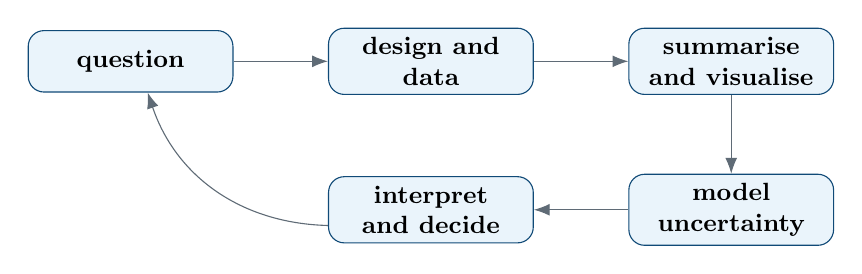
\begin{tikzpicture}[node distance=10mm and 12mm, every node/.style={font=\small\bfseries,align=center},
  s/.style={rounded corners=2mm,draw=blue!70!black,fill=bluepale,minimum width=2.6cm,minimum height=0.78cm},
  a/.style={-{Latex[length=2mm]},draw=muted}]
  \node[s] (q) {question};
  \node[s,right=of q] (d) {design and\\data};
  \node[s,right=of d] (sum) {summarise\\and visualise};
  \node[s,below=of sum] (model) {model\\uncertainty};
  \node[s,left=of model] (dec) {interpret\\and decide};
  \draw[a] (q)--(d); \draw[a] (d)--(sum); \draw[a] (sum)--(model); \draw[a] (model)--(dec); \draw[a] (dec) to[bend left=35] (q);
\end{tikzpicture}
\end{center}

\section{Centre and spread}

The mean is the balancing point:
\[
  \bar x=\frac{1}{n}\sum_{i=1}^n x_i.
\]
The median is the middle value after sorting. The range is maximum minus minimum. The standard deviation is the typical distance from the mean, with the precise denominator depending on whether we describe a population or estimate from a sample.

\begin{center}
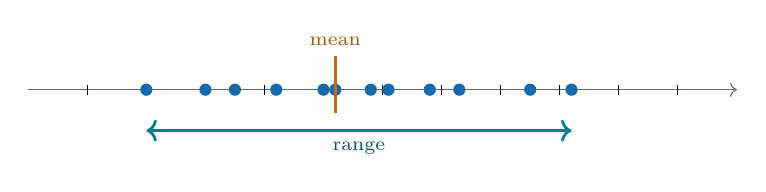
\begin{tikzpicture}[x=0.75cm,y=0.65cm]
  \draw[->,muted] (0,0)--(12,0);
  \foreach \x in {1,...,11}{\draw (\x,0.1)--(\x,-0.1);}
  \foreach \x in {2,3,3.5,4.2,5,5.2,5.8,6.1,6.8,7.3,8.5,9.2}{\fill[blue] (\x,0) circle (2.2pt);}
  \draw[orange,line width=1.2pt] (5.2,-0.45)--(5.2,0.65);
  \draw[teal,<->,line width=1pt] (2,-0.8)--(9.2,-0.8);
  \node[font=\scriptsize,orange!80!black] at (5.2,0.95) {mean};
  \node[font=\scriptsize,teal!70!black] at (5.6,-1.15) {range};
\end{tikzpicture}
\end{center}

\section{Correlation and regression}

Correlation describes the strength and direction of a linear association. It does not prove that one variable causes the other. A simple regression line predicts $y$ from $x$:
\[
  \hat y=\hat\beta_0+\hat\beta_1x.
\]
The slope is the predicted change in $y$ for a one-unit increase in $x$, under the model and its assumptions.

\begin{center}
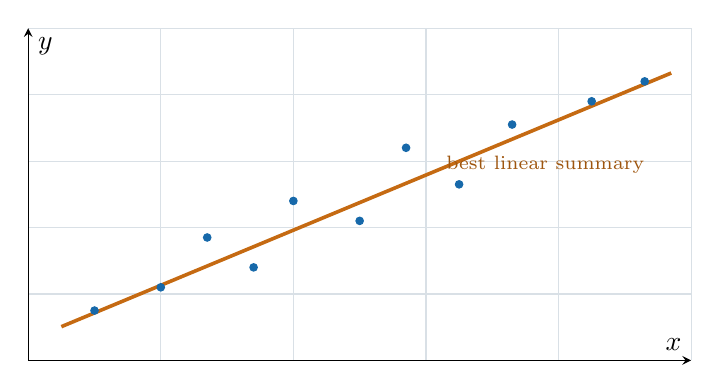
\begin{tikzpicture}
\begin{axis}[width=10cm,height=5.8cm,axis lines=middle,xmin=0,xmax=10,ymin=0,ymax=10,grid=both,major grid style={draw=linegray},ticks=none,xlabel={$x$},ylabel={$y$}]
  \addplot[only marks,mark=*,blue,mark size=1.35pt] coordinates {(1,1.5)(2,2.2)(2.7,3.7)(3.4,2.8)(4,4.8)(5,4.2)(5.7,6.4)(6.5,5.3)(7.3,7.1)(8.5,7.8)(9.3,8.4)};
  \addplot[orange,line width=1.3pt,domain=0.5:9.7]{0.83*x+0.6};
  \node[font=\scriptsize,orange!80!black] at (7.8,5.9) {best linear summary};
\end{axis}
\end{tikzpicture}
\end{center}

\section{Sampling, uncertainty, and confidence intervals}

A sample is used because observing every member of a population is often impossible. A statistic such as $\bar x$ varies from sample to sample. A confidence interval is a procedure that, over repeated samples, captures the target parameter at a stated rate under its assumptions. It is not a probability statement about a fixed parameter after the interval is computed.

\begin{center}
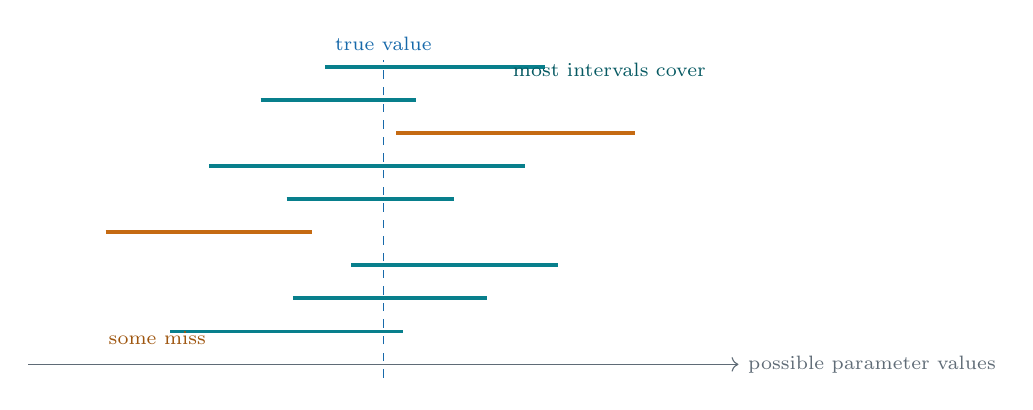
\begin{tikzpicture}[x=0.82cm,y=0.42cm]
  \draw[->,muted] (0,0)--(11,0) node[right,font=\scriptsize] {possible parameter values};
  \draw[blue,dashed] (5.5,-0.4)--(5.5,9.2) node[above,font=\scriptsize] {true value};
  \foreach \y/\a/\b in {1/2.2/5.8,2/4.1/7.1,3/5.0/8.2,5/4.0/6.6,6/2.8/7.7,8/3.6/6.0,9/4.6/8.0}
    {\draw[teal,line width=1.3pt] (\a,\y)--(\b,\y);}
  \foreach \y/\a/\b in {4/1.2/4.4,7/5.7/9.4}
    {\draw[orange,line width=1.3pt] (\a,\y)--(\b,\y);}
  \node[font=\scriptsize,teal!70!black] at (9,8.9) {most intervals cover};
  \node[font=\scriptsize,orange!80!black] at (2,0.8) {some miss};
\end{tikzpicture}
\end{center}

\section{Causality is a design problem}

Association asks whether variables move together. Causality asks what would happen to the same unit under a different treatment. Randomisation balances confounders in expectation. Observational designs need assumptions such as no unmeasured confounding, parallel trends, or a valid instrument.

\begin{center}
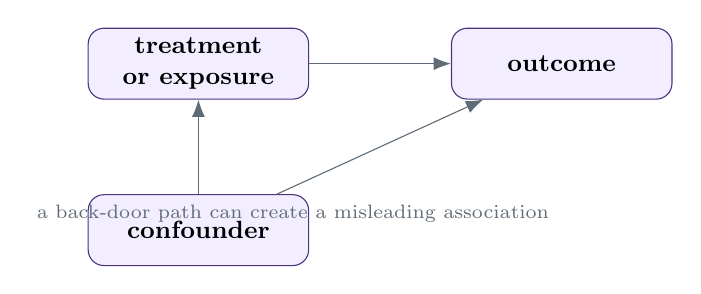
\begin{tikzpicture}[node distance=12mm and 18mm, every node/.style={font=\small\bfseries,align=center},
  s/.style={rounded corners=2mm,draw=purple!70!black,fill=purplepale,minimum width=2.8cm,minimum height=0.9cm},
  a/.style={-{Latex[length=2.2mm]},draw=muted}]
  \node[s] (t) {treatment\\or exposure};
  \node[s,right=of t] (y) {outcome};
  \node[s,below=of t] (c) {confounder};
  \draw[a] (t)--(y);
  \draw[a] (c)--(t); \draw[a] (c)--(y);
  \node[font=\scriptsize,muted] at (1.2,-1.9) {a back-door path can create a misleading association};
\end{tikzpicture}
\end{center}

\chapter{Logic, proof, and discrete mathematics}

\section{Statements and logical connectors}

A proposition is a statement that is true or false. Negation reverses truth. Conjunction ``and'' is true only when both parts are true; disjunction ``or'' is true when at least one part is true; implication $P\Rightarrow Q$ says that whenever $P$ is true, $Q$ must be true.

\begin{center}
\begin{tabular}{c c c c}
\toprule
$P$ & $Q$ & $P\land Q$ & $P\Rightarrow Q$\\
\midrule
T&T&T&T\\
T&F&F&F\\
F&T&F&T\\
F&F&F&T\\
\bottomrule
\end{tabular}
\end{center}

The implication is only false when the premise is true and the conclusion is false. This can feel surprising because an implication is a rule about a case, not a claim that the premise actually occurs.

\section{Sets and functions}

Sets collect objects. Union $A\cup B$ combines them; intersection $A\cap B$ keeps what they share; complement $A^c$ keeps what lies outside. A function is a special relation that assigns one output to each input. Injective means no two inputs collide; surjective means every target is reached; bijective means both.

\begin{center}
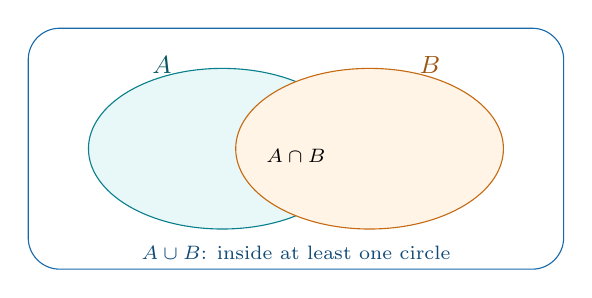
\begin{tikzpicture}[scale=0.85]
  \draw[blue,rounded corners=4mm] (-4,-1.8) rectangle (4,1.8);
  \draw[fill=tealpale,draw=teal] (-1.1,0) ellipse (2.0 and 1.2);
  \draw[fill=orangepale,draw=orange] (1.1,0) ellipse (2.0 and 1.2);
  \node[font=\small\bfseries,teal!70!black] at (-2.0,1.25) {$A$};
  \node[font=\small\bfseries,orange!80!black] at (2.0,1.25) {$B$};
  \node[font=\scriptsize] at (0,-0.1) {$A\cap B$};
  \node[font=\scriptsize,blue!70!black] at (0,-1.55) {$A\cup B$: inside at least one circle};
\end{tikzpicture}
\end{center}

\section{Direct proof, contradiction, and induction}

A direct proof starts with the assumptions and derives the conclusion. A proof by contradiction assumes the conclusion is false and derives an impossibility. Mathematical induction proves a statement for every natural number by showing a base case and a step from $n$ to $n+1$.

\begin{center}
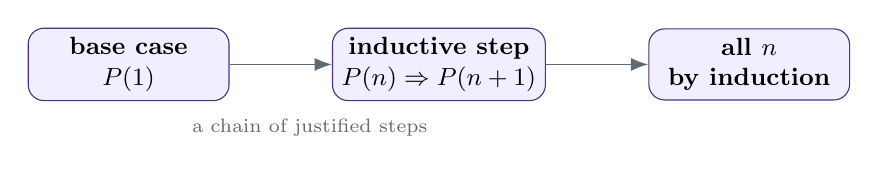
\begin{tikzpicture}[node distance=11mm and 13mm, every node/.style={font=\small\bfseries,align=center},
  s/.style={rounded corners=2mm,draw=purple!70!black,fill=purplepale,minimum width=2.55cm,minimum height=0.8cm},
  a/.style={-{Latex[length=2.2mm]},draw=muted}]
  \node[s] (base) {base case\\$P(1)$};
  \node[s,right=of base] (step) {inductive step\\$P(n)\Rightarrow P(n+1)$};
  \node[s,right=of step] (all) {all $n$\\by induction};
  \draw[a] (base)--(step); \draw[a] (step)--(all);
  \node[font=\scriptsize,muted] at (2.3,-0.8) {a chain of justified steps};
\end{tikzpicture}
\end{center}

\begin{proofbox}{Example: sum of the first $n$ odd numbers}
For $n=1$, the sum is $1=1^2$. Suppose $1+3+\cdots+(2n-1)=n^2$. Adding the next odd number gives
\[
  n^2+(2n+1)=(n+1)^2.
\]
Therefore the statement holds for every $n\in\N$:
\[
  1+3+5+\cdots+(2n-1)=n^2.
\]
The algebra works because the next square is exactly the previous square plus the next odd number.
\end{proofbox}

\section{Counting and combinatorics}

The multiplication principle says that if a task has $a$ choices followed by $b$ choices, there are $ab$ combined choices. Arrangements of $n$ distinct objects count as $n!$. Choosing $k$ objects without caring about order gives
\[
  \binom{n}{k}=\frac{n!}{k!(n-k)!}.
\]
These coefficients form Pascal's triangle and appear in the binomial theorem:
\[
  (a+b)^n=\sum_{k=0}^n \binom{n}{k}a^{n-k}b^k.
\]

\begin{center}
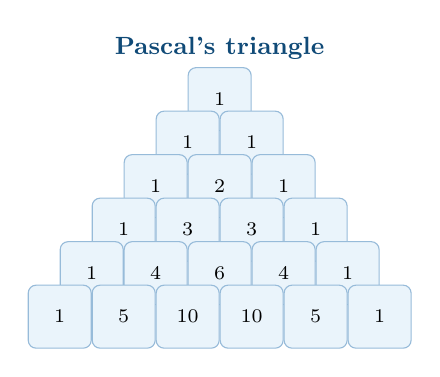
\begin{tikzpicture}[scale=0.65]
  \foreach \r in {0,...,5}{
    \foreach \c in {0,...,\r}{
      \pgfmathtruncatemacro{\val}{\c==0 || \c==\r ? 1 : 0}
      \ifnum\r>1
        \pgfmathtruncatemacro{\val}{int(factorial(\r)/(factorial(\c)*factorial(\r-\c)))}
      \fi
      \node[draw=blue!45,fill=bluepale,rounded corners=1mm,minimum size=8mm,font=\scriptsize] at ({(\c-\r/2)*1.25},{-\r*0.85}) {\val};
    }
  }
  \node[font=\small\bfseries,blue!70!black] at (0,1.0) {Pascal's triangle};
\end{tikzpicture}
\end{center}

\section{Graphs and networks}

In discrete mathematics, a graph is a set of vertices connected by edges. Degree counts how many edges touch a vertex. Paths describe movement through a network; cycles return to their starting point. Graphs model roads, friendships, computer networks, dependencies, and state transitions.

\begin{center}
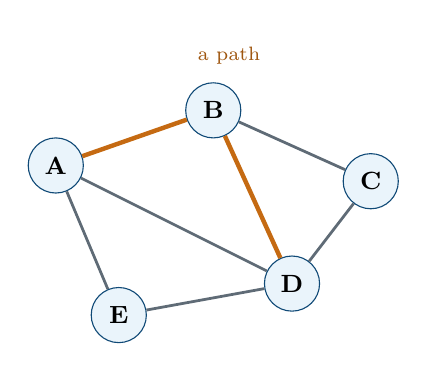
\begin{tikzpicture}[every node/.style={circle,draw=blue!70!black,fill=bluepale,minimum size=7mm,font=\small\bfseries},
  e/.style={draw=muted,line width=1pt}]
  \node (a) at (0,1.5) {A}; \node (b) at (2,2.2) {B}; \node (c) at (4,1.3) {C}; \node (d) at (3,0) {D}; \node (e2) at (0.8,-0.4) {E};
  \draw[e] (a)--(b)--(c)--(d)--(a)--(e2)--(d); \draw[e] (b)--(d); \draw[e,orange,line width=1.6pt] (a)--(b)--(d);
  \node[font=\scriptsize,draw=none,fill=none,shape=rectangle,orange!80!black] at (2.2,2.9) {a path};
\end{tikzpicture}
\end{center}

\chapter{Differential equations and dynamical systems}

\section{Equations for change}

An algebraic equation asks for a number. A differential equation asks for a function whose derivatives satisfy a rule. The equation
\[
  \frac{\dd y}{\dd t}=ky
\]
says that the rate of change is proportional to the current amount. Its solutions are $y(t)=Ce^{kt}$, which explains why exponentials appear in growth, decay, cooling, finance, and population models.

\begin{center}
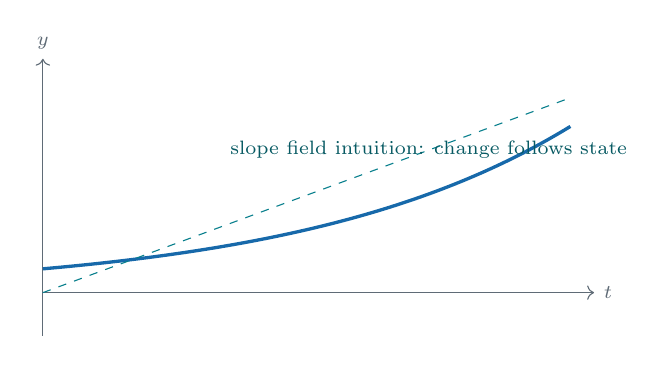
\begin{tikzpicture}[x=1.0cm,y=0.55cm]
  \draw[->,muted] (0,0)--(7,0) node[right,font=\scriptsize] {$t$};
  \draw[->,muted] (0,-1)--(0,5.4) node[above,font=\scriptsize] {$y$};
  \draw[blue,line width=1.2pt,samples=100,domain=0:6.7] plot (\x,{0.55*exp(0.29*\x)});
  \draw[teal,dashed] (0,0)--(6.7,4.5);
  \node[font=\scriptsize,teal!70!black] at (4.9,3.3) {slope field intuition: change follows state};
\end{tikzpicture}
\end{center}

\section{Phase space and stability}

For a system with several changing variables, phase space records the current state. A trajectory shows how the state evolves. An equilibrium is a state that does not move. It is stable if nearby trajectories stay close or return; unstable if nearby trajectories move away.

\begin{center}
\begin{tikzpicture}[x=1cm,y=1cm]
  \draw[->,muted] (-3.2,0)--(3.3,0) node[right,font=\scriptsize] {$x$};
  \draw[->,muted] (0,-2.5)--(0,2.8) node[above,font=\scriptsize] {$v$};
  \foreach \x in {-2.6,-1.8,-1.0,1.0,1.8,2.6}{\draw[->,blue!55] (\x,1.8)--({0.8*\x},0.8); \draw[->,blue!55] (\x,-1.8)--({0.8*\x},-0.8);}
  \draw[teal,line width=1.6pt] (0,0) circle (2pt);
  \node[font=\small,teal!70!black] at (1.55,-1.9) {stable equilibrium};
\end{tikzpicture}
\end{center}

\section{Discrete-time systems and feedback}

An iteration $x_{n+1}=f(x_n)$ repeatedly applies a rule. Feedback can settle to a fixed point, oscillate, or become chaotic. The logistic map
\[
  x_{n+1}=rx_n(1-x_n)
\]
shows how a simple rule can generate rich behaviour as the parameter $r$ changes.

\begin{center}
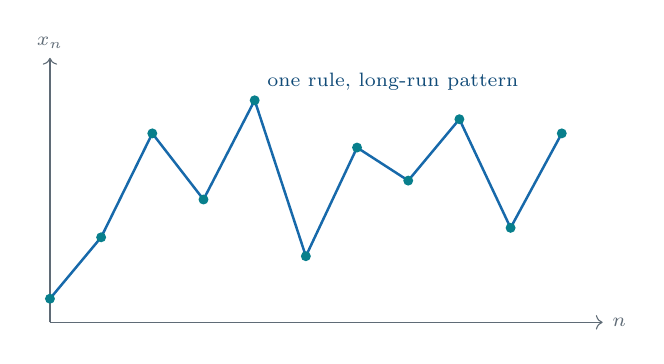
\begin{tikzpicture}[x=0.65cm,y=0.6cm]
  \draw[->,muted] (0,0)--(10.8,0) node[right,font=\scriptsize] {$n$};
  \draw[->,muted] (0,0)--(0,5.6) node[above,font=\scriptsize] {$x_n$};
  \draw[blue,line width=0.9pt] plot coordinates {(0,0.5)(1,1.8)(2,4.0)(3,2.6)(4,4.7)(5,1.4)(6,3.7)(7,3.0)(8,4.3)(9,2.0)(10,4.0)};
  \foreach \x/\y in {0/0.5,1/1.8,2/4.0,3/2.6,4/4.7,5/1.4,6/3.7,7/3.0,8/4.3,9/2.0,10/4.0}{\fill[teal] (\x,\y) circle (1.8pt);}
  \node[font=\scriptsize,blue!70!black] at (6.7,5.1) {one rule, long-run pattern};
\end{tikzpicture}
\end{center}

\chapter{Optimisation and numerical thinking}

\section{The geometry of an optimum}

Optimisation asks for the best feasible value: smallest cost, largest area, shortest route, or highest expected utility. A model has an objective function and constraints. The feasible region contains the choices allowed by the constraints.

\begin{center}
\begin{tikzpicture}[x=0.9cm,y=0.9cm]
  \draw[->,muted] (-0.2,0)--(6.2,0) node[right,font=\scriptsize] {$x$};
  \draw[->,muted] (0,-0.2)--(0,5.7) node[above,font=\scriptsize] {$y$};
  \fill[tealpale] (0,0)--(4.8,0)--(2.4,3.4)--(0,4.7)--cycle;
  \draw[teal,line width=1pt] (0,0)--(4.8,0)--(2.4,3.4)--(0,4.7)--cycle;
  \foreach \r in {0.7,1.4,2.1,2.8}{\draw[blue!55] (\r,0.3)--(\r+2.1,4.1);}
  \fill[orange] (4.8,0) circle (2.5pt);
  \node[font=\scriptsize,teal!70!black] at (1.7,2.1) {feasible region};
  \node[font=\scriptsize,orange!80!black] at (5.3,0.5) {candidate optimum};
\end{tikzpicture}
\end{center}

Linear programming is special because both the objective and constraints are linear. An optimum, when it exists, occurs at a corner of the feasible polytope. Nonlinear optimisation uses derivatives, convexity, or iterative algorithms.

\section{Numerical approximation}

Many equations cannot be solved in closed form. Numerical methods replace an exact answer with a controlled approximation. Newton's method uses the tangent line to improve a guess:
\[
  x_{n+1}=x_n-\frac{f(x_n)}{f'(x_n)}.
\]
The method can be fast near a good root, but it can diverge or jump to a different root when the starting point is poor.

\begin{center}
\begin{tikzpicture}[x=1.05cm,y=0.75cm]
  \draw[->,muted] (-2.6,0)--(3.2,0); \draw[->,muted] (0,-1.3)--(0,4.7);
  \draw[blue,line width=1.2pt,samples=100,domain=-2.1:2.4] plot (\x,{0.55*(\x-1.4)*(\x-1.4)-0.4});
  \draw[orange,line width=0.9pt] (-0.3,2.0)--(1.55,-0.4);
  \draw[teal,dashed] (-0.3,0)--(-0.3,2.0); \draw[teal,dashed] (1.55,0)--(1.55,-0.4);
  \fill[orange] (-0.3,2.0) circle (2.2pt); \fill[teal] (1.55,-0.4) circle (2.2pt);
  \node[font=\scriptsize,orange!80!black] at (-0.8,2.5) {guess};
  \node[font=\scriptsize,teal!70!black] at (1.9,0.2) {next guess};
\end{tikzpicture}
\end{center}

\section{Error and scale}

The absolute error is $\abs{\text{approximation}-\text{truth}}$. Relative error divides by the size of the truth. Significant digits communicate precision without pretending that every digit is equally reliable. Good numerical work reports assumptions, units, conditioning, and a stopping rule.

\chapter{The higher-mathematics landscape}

\section{The same patterns keep returning}

Advanced mathematics often feels new because the objects become abstract. The underlying questions are familiar:

\begin{center}
\begin{tabular}{>{\bfseries}p{0.25\linewidth} p{0.66\linewidth}}
\toprule
Pattern & Mathematical language \\
\midrule
Change & derivative, difference equation, dynamical system \\
Accumulation & sum, integral, measure, expectation \\
Symmetry & group, transformation, invariant \\
Nearness & metric, topology, continuity, convergence \\
Structure & algebraic operation, vector space, category \\
Uncertainty & probability measure, random variable, stochastic process \\
Optimality & objective, constraint, convexity, variational principle \\
\bottomrule
\end{tabular}
\end{center}

\section{Abstract algebra}

A group is a set with an operation satisfying closure, associativity, an identity, and inverses. Integers under addition form a group. Rotations of a square form a finite group. The common idea is that we can compose transformations and undo them.

\begin{center}
\begin{tikzpicture}[node distance=13mm, every node/.style={font=\small\bfseries,align=center},
  s/.style={rounded corners=2mm,draw=blue!70!black,fill=bluepale,minimum width=2.8cm,minimum height=0.82cm},
  a/.style={-{Latex[length=2.2mm]},draw=muted}]
  \node[s] (obj) {objects};
  \node[s,right=of obj] (op) {operation\\combine};
  \node[s,right=of op] (law) {laws\\invariants};
  \draw[a] (obj)--(op); \draw[a] (op)--(law);
  \node[font=\scriptsize,muted] at (2.6,-0.9) {abstract algebra studies composition};
\end{tikzpicture}
\end{center}

Rings support addition and multiplication. Fields allow division by every nonzero element. Linear algebra is built over a field, commonly $\R$ or $\C$.

\section{Topology and continuity}

Topology studies properties preserved by continuous deformation: connectedness, holes, boundaries, and convergence. A topological space specifies which sets count as open, allowing a rigorous notion of continuity without requiring ordinary distance coordinates.

\begin{center}
\begin{tikzpicture}[scale=0.8]
  \draw[blue,line width=1.2pt] (-4,0) ellipse (1.35 and 1.0);
  \draw[teal,line width=1.2pt] (0,0) ellipse (1.45 and 1.0);
  \draw[orange,line width=1.2pt] (4,0) ellipse (1.55 and 1.0);
  \draw[white,line width=3pt] (4,0.8) ellipse (0.55 and 0.3);
  \node[font=\small\bfseries,blue!70!black] at (-4,-1.55) {disk};
  \node[font=\small\bfseries,teal!70!black] at (0,-1.55) {sphere surface};
  \node[font=\small\bfseries,orange!80!black] at (4,-1.55) {torus};
  \node[font=\scriptsize,muted] at (0,1.55) {number of holes is a topological invariant};
\end{tikzpicture}
\end{center}

\section{Measure and modern probability}

Measure theory generalises length, area, and volume. It provides a careful foundation for integration and probability, especially when outcomes are continuous or infinite. A probability measure assigns total mass $1$ to the sample space and supports expectation as an integral.

\section{Fourier analysis and signals}

Fourier analysis represents a complicated periodic signal as a combination of simple sines and cosines. Frequencies are to signals what coordinates are to positions: a different but useful representation.

\begin{center}
\begin{tikzpicture}[x=0.72cm,y=0.62cm]
  \draw[->,muted] (0,0)--(14,0) node[right,font=\scriptsize] {time};
  \draw[->,muted] (0,-2.4)--(0,2.6) node[above,font=\scriptsize] {signal};
  \draw[blue,line width=1pt,samples=150,domain=0:13.4] plot (\x,{0.95*sin(42*\x)+0.5*sin(105*\x)});
  \draw[orange,dashed,line width=0.8pt,samples=150,domain=0:13.4] plot (\x,{0.95*sin(42*\x)});
  \node[font=\scriptsize,blue!70!black] at (10.3,2.1) {sum of frequencies};
  \node[font=\scriptsize,orange!80!black] at (10.5,-1.8) {one component};
\end{tikzpicture}
\end{center}

\section{A practical route through mathematics}

\begin{center}
\begin{tikzpicture}[node distance=8mm and 6mm, every node/.style={font=\scriptsize\bfseries,align=center},
  s/.style={rounded corners=2mm,draw=blue!70!black,fill=bluepale,minimum width=2.15cm,minimum height=0.65cm},
  a/.style={-{Latex[length=2mm]},draw=muted}]
  \node[s] (a) {arithmetic};
  \node[s,right=of a] (b) {algebra};
  \node[s,right=of b] (c) {functions};
  \node[s,right=of c] (d) {calculus};
  \node[s,below=of b] (e) {geometry};
  \node[s,right=of e] (f) {linear algebra};
  \node[s,right=of f] (g) {probability};
  \node[s,right=of g] (h) {statistics};
  \node[s,below=of f] (i) {proof and discrete math};
  \node[s,right=of i] (j) {modelling and computation};
  \draw[a] (a)--(b)--(c)--(d); \draw[a] (e)--(f)--(g)--(h); \draw[a] (b)--(e); \draw[a] (c)--(f); \draw[a] (d)--(j); \draw[a] (h)--(j); \draw[a] (i)--(j); \draw[a] (f)--(i);
\end{tikzpicture}
\end{center}

\chapter{Reference: formulas as connected ideas}

\section{Algebra and geometry}
\begin{multicols}{2}
\begin{itemize}
  \item Distributive law: $a(b+c)=ab+ac$.
  \item Difference of squares: $a^2-b^2=(a-b)(a+b)$.
  \item Quadratic formula: $x=(-b\pm\sqrt{b^2-4ac})/(2a)$.
  \item Distance: $d=\sqrt{(x_2-x_1)^2+(y_2-y_1)^2}$.
  \item Circle: $A=\pi r^2$, $C=2\pi r$.
  \item Triangle: $A=\frac12 bh$.
  \item Sphere: $V=\frac43\pi r^3$.
  \item Pythagoras: $a^2+b^2=c^2$.
\end{itemize}
\end{multicols}

\section{Trigonometry and calculus}
\begin{multicols}{2}
\begin{itemize}
  \item $\sin^2\theta+\cos^2\theta=1$.
  \item $\sin(\alpha+\beta)=\sin\alpha\cos\beta+\cos\alpha\sin\beta$.
  \item Derivative: $\frac{\dd}{\dd x}x^n=nx^{n-1}$.
  \item Product: $(fg)'=f'g+fg'$.
  \item Chain: $(f(g(x)))'=f'(g(x))g'(x)$.
  \item Exponential: $(e^x)'=e^x$.
  \item Integral: $\int x^n\dd x=x^{n+1}/(n+1)+C$.
  \item Fundamental theorem: $\int_a^b f=F(b)-F(a)$.
\end{itemize}
\end{multicols}

\section{Probability and statistics}
\begin{multicols}{2}
\begin{itemize}
  \item Complement: $P(A^c)=1-P(A)$.
  \item Conditional: $P(A\mid B)=P(A\cap B)/P(B)$.
  \item Independence: $P(A\cap B)=P(A)P(B)$.
  \item Expected value: $\mathbb{E}X=\sum_xxP(X=x)$.
  \item Variance: $\operatorname{Var}(X)=\mathbb{E}[(X-\mathbb{E}X)^2]$.
  \item Mean: $\bar x=\sum x_i/n$.
  \item Covariance: $\operatorname{Cov}(X,Y)=\mathbb{E}[(X-\mu_X)(Y-\mu_Y)]$.
  \item Standard score: $z=(x-\mu)/\sigma$.
\end{itemize}
\end{multicols}

\section{Linear algebra and discrete mathematics}
\begin{multicols}{2}
\begin{itemize}
  \item Dot product: $\vect u\cdot\vect v=\sum u_iv_i$.
  \item Norm: $\norm{\vect v}=\sqrt{\vect v\cdot\vect v}$.
  \item Linear system: $A\vect x=\vect b$.
  \item Eigenvector: $A\vect v=\lambda\vect v$.
  \item Determinant: signed area or volume scale.
  \item Factorial: $n!=n(n-1)\cdots1$.
  \item Combination: $\binom{n}{k}=n!/[k!(n-k)!]$.
  \item Induction: base case plus $P(n)\Rightarrow P(n+1)$.
\end{itemize}
\end{multicols}

\chapter*{Final perspective}
\addcontentsline{toc}{chapter}{Final perspective}

The most powerful habit in mathematics is to ask what an expression is doing. Is it counting? Measuring distance? Describing a map? Accumulating change? Assigning probability? Encoding a constraint? Proving that a pattern cannot fail?

When a formula feels opaque, translate it three ways:

\begin{enumerate}
  \item draw the object or relationship;
  \item say the formula in ordinary language;
  \item test it on the smallest example that could work.
\end{enumerate}

Then ask what changes when an input changes. That question is the bridge from arithmetic to algebra, from algebra to calculus, from geometry to linear algebra, and from probability to statistics. Mathematics becomes a connected subject when the symbols are allowed to point back to the structures they describe.

\begin{center}
\begin{tikzpicture}[scale=0.85]
  \draw[->,blue,line width=1.3pt] (-3.2,0)--(3.4,0) node[right,font=\small] {structure};
  \draw[->,teal,line width=1.3pt] (0,-2.2)--(0,2.8) node[above,font=\small] {representation};
  \draw[orange,line width=1.2pt] (-2.5,-1.2)--(2.5,2.0);
  \node[font=\small\bfseries,blue!70!black] at (-2.2,0.38) {notice};
  \node[font=\small\bfseries,teal!70!black] at (0.55,2.0) {name};
  \node[font=\small\bfseries,orange!80!black] at (2.3,-0.35) {use};
\end{tikzpicture}
\end{center}

\vfill
\begin{center}
\textcolor{muted}{\small End of the visual roadmap}\par
\textcolor{muted}{\small Scott Brodie Forsyth \textbullet\ 2026}
\end{center}

\end{document}